\documentclass[twoside]{book}

% Packages required by doxygen
\usepackage{fixltx2e}
\usepackage{calc}
\usepackage{doxygen}
\usepackage[export]{adjustbox} % also loads graphicx
\usepackage{graphicx}
\usepackage[utf8]{inputenc}
\usepackage{makeidx}
\usepackage{multicol}
\usepackage{multirow}
\PassOptionsToPackage{warn}{textcomp}
\usepackage{textcomp}
\usepackage[nointegrals]{wasysym}
\usepackage[table]{xcolor}

% Font selection
\usepackage[T1]{fontenc}
\usepackage[scaled=.90]{helvet}
\usepackage{courier}
\usepackage{amssymb}
\usepackage{sectsty}
\renewcommand{\familydefault}{\sfdefault}
\allsectionsfont{%
  \fontseries{bc}\selectfont%
  \color{darkgray}%
}
\renewcommand{\DoxyLabelFont}{%
  \fontseries{bc}\selectfont%
  \color{darkgray}%
}
\newcommand{\+}{\discretionary{\mbox{\scriptsize$\hookleftarrow$}}{}{}}

% Page & text layout
\usepackage{geometry}
\geometry{%
  letterpaper,%
  top=2.5cm,%
  bottom=2.5cm,%
  left=2.5cm,%
  right=2.5cm%
}
\tolerance=750
\hfuzz=15pt
\hbadness=750
\setlength{\emergencystretch}{15pt}
\setlength{\parindent}{0cm}
\setlength{\parskip}{3ex plus 2ex minus 2ex}
\makeatletter
\renewcommand{\paragraph}{%
  \@startsection{paragraph}{4}{0ex}{-1.0ex}{1.0ex}{%
    \normalfont\normalsize\bfseries\SS@parafont%
  }%
}
\renewcommand{\subparagraph}{%
  \@startsection{subparagraph}{5}{0ex}{-1.0ex}{1.0ex}{%
    \normalfont\normalsize\bfseries\SS@subparafont%
  }%
}
\makeatother

% Headers & footers
\usepackage{fancyhdr}
\pagestyle{fancyplain}
\fancyhead[LE]{\fancyplain{}{\bfseries\thepage}}
\fancyhead[CE]{\fancyplain{}{}}
\fancyhead[RE]{\fancyplain{}{\bfseries\leftmark}}
\fancyhead[LO]{\fancyplain{}{\bfseries\rightmark}}
\fancyhead[CO]{\fancyplain{}{}}
\fancyhead[RO]{\fancyplain{}{\bfseries\thepage}}
\fancyfoot[LE]{\fancyplain{}{}}
\fancyfoot[CE]{\fancyplain{}{}}
\fancyfoot[RE]{\fancyplain{}{\bfseries\scriptsize Generated by Doxygen }}
\fancyfoot[LO]{\fancyplain{}{\bfseries\scriptsize Generated by Doxygen }}
\fancyfoot[CO]{\fancyplain{}{}}
\fancyfoot[RO]{\fancyplain{}{}}
\renewcommand{\footrulewidth}{0.4pt}
\renewcommand{\chaptermark}[1]{%
  \markboth{#1}{}%
}
\renewcommand{\sectionmark}[1]{%
  \markright{\thesection\ #1}%
}

% Indices & bibliography
\usepackage{natbib}
\usepackage[titles]{tocloft}
\setcounter{tocdepth}{3}
\setcounter{secnumdepth}{5}
\makeindex

% Packages requested by user
\usepackage{amsmath}

% Hyperlinks (required, but should be loaded last)
\usepackage{ifpdf}
\ifpdf
  \usepackage[pdftex,pagebackref=true]{hyperref}
\else
  \usepackage[ps2pdf,pagebackref=true]{hyperref}
\fi
\hypersetup{%
  colorlinks=true,%
  linkcolor=blue,%
  citecolor=blue,%
  unicode%
}

% Custom commands
\newcommand{\clearemptydoublepage}{%
  \newpage{\pagestyle{empty}\cleardoublepage}%
}

\usepackage{caption}
\captionsetup{labelsep=space,justification=centering,font={bf},singlelinecheck=off,skip=4pt,position=top}

%===== C O N T E N T S =====

\begin{document}

% Titlepage & ToC
\hypersetup{pageanchor=false,
             bookmarksnumbered=true,
             pdfencoding=unicode
            }
\pagenumbering{alph}
\begin{titlepage}
\vspace*{7cm}
\begin{center}%
{\Large Video\+\_\+\+Store \\[1ex]\large 1.\+0 }\\
\vspace*{1cm}
{\large Generated by Doxygen 1.8.13}\\
\end{center}
\end{titlepage}
\clearemptydoublepage
\pagenumbering{roman}
\tableofcontents
\clearemptydoublepage
\pagenumbering{arabic}
\hypersetup{pageanchor=true}

%--- Begin generated contents ---
\chapter{Namespace Index}
\section{Packages}
Here are the packages with brief descriptions (if available)\+:\begin{DoxyCompactList}
\item\contentsline{section}{\hyperlink{namespaceAbstractItem}{Abstract\+Item} \\*Partial implementation of the \hyperlink{namespaceItem}{Item} interface }{\pageref{namespaceAbstractItem}}{}
\item\contentsline{section}{\hyperlink{namespaceCustomer}{Customer} \\*A class describing a customer of the Video Store }{\pageref{namespaceCustomer}}{}
\item\contentsline{section}{\hyperlink{namespaceGenreSearch}{Genre\+Search} \\*Class for searching items matching a given genre }{\pageref{namespaceGenreSearch}}{}
\item\contentsline{section}{\hyperlink{namespaceItem}{Item} \\*A class modeling an item of the Video Store }{\pageref{namespaceItem}}{}
\item\contentsline{section}{\hyperlink{namespaceSearchCondition}{Search\+Condition} \\*A search predicate for items }{\pageref{namespaceSearchCondition}}{}
\item\contentsline{section}{\hyperlink{namespaceSimpleDate}{Simple\+Date} \\*Packages dates in the format yyyy-\/mm-\/dd }{\pageref{namespaceSimpleDate}}{}
\item\contentsline{section}{\hyperlink{namespaceStatusException}{Status\+Exception} \\*Exceptions to be thrown when an error has occurred }{\pageref{namespaceStatusException}}{}
\item\contentsline{section}{\hyperlink{namespaceVideoStore}{Video\+Store} \\*A video store that rents D\+V\+Ds, and Games }{\pageref{namespaceVideoStore}}{}
\end{DoxyCompactList}

\chapter{Hierarchical Index}
\section{Class Hierarchy}
This inheritance list is sorted roughly, but not completely, alphabetically\+:\begin{DoxyCompactList}
\item \contentsline{section}{Customer.\+Customer}{\pageref{classCustomer_1_1Customer}}{}
\item Exception\begin{DoxyCompactList}
\item \contentsline{section}{Status\+Exception.\+Status\+Exception}{\pageref{classStatusException_1_1StatusException}}{}
\end{DoxyCompactList}
\item object\begin{DoxyCompactList}
\item \contentsline{section}{Item.\+Item}{\pageref{classItem_1_1Item}}{}
\begin{DoxyCompactList}
\item \contentsline{section}{Abstract\+Item.\+Abstract\+Item}{\pageref{classAbstractItem_1_1AbstractItem}}{}
\end{DoxyCompactList}
\end{DoxyCompactList}
\item \contentsline{section}{Search\+Condition.\+Search\+Condition}{\pageref{classSearchCondition_1_1SearchCondition}}{}
\begin{DoxyCompactList}
\item \contentsline{section}{Genre\+Search.\+Genre\+Search}{\pageref{classGenreSearch_1_1GenreSearch}}{}
\end{DoxyCompactList}
\item \contentsline{section}{Simple\+Date.\+Simple\+Date}{\pageref{classSimpleDate_1_1SimpleDate}}{}
\item \contentsline{section}{Video\+Store.\+Video\+Store}{\pageref{classVideoStore_1_1VideoStore}}{}
\end{DoxyCompactList}

\chapter{Class Index}
\section{Class List}
Here are the classes, structs, unions and interfaces with brief descriptions\+:\begin{DoxyCompactList}
\item\contentsline{section}{\hyperlink{classAbstractItem_1_1AbstractItem}{Abstract\+Item.\+Abstract\+Item} \\*Partial implementation of the \hyperlink{namespaceItem}{Item} interface }{\pageref{classAbstractItem_1_1AbstractItem}}{}
\item\contentsline{section}{\hyperlink{classCustomer_1_1Customer}{Customer.\+Customer} \\*A \hyperlink{classCustomer_1_1Customer}{Customer} is a client of a \hyperlink{namespaceVideoStore}{Video\+Store} who can rent items }{\pageref{classCustomer_1_1Customer}}{}
\item\contentsline{section}{\hyperlink{classGenreSearch_1_1GenreSearch}{Genre\+Search.\+Genre\+Search} \\*Implementation of \hyperlink{namespaceSearchCondition}{Search\+Condition} that matches items based on the genre (not case sensitive) }{\pageref{classGenreSearch_1_1GenreSearch}}{}
\item\contentsline{section}{\hyperlink{classItem_1_1Item}{Item.\+Item} \\*This is an abstract class }{\pageref{classItem_1_1Item}}{}
\item\contentsline{section}{\hyperlink{classSearchCondition_1_1SearchCondition}{Search\+Condition.\+Search\+Condition} \\*Abstraction of a search predicate for items }{\pageref{classSearchCondition_1_1SearchCondition}}{}
\item\contentsline{section}{\hyperlink{classSimpleDate_1_1SimpleDate}{Simple\+Date.\+Simple\+Date} \\*Date consisting of a year, month, and day }{\pageref{classSimpleDate_1_1SimpleDate}}{}
\item\contentsline{section}{\hyperlink{classStatusException_1_1StatusException}{Status\+Exception.\+Status\+Exception} \\*Exception type thrown for invalid operations such as attempting to rent an item that is already rented }{\pageref{classStatusException_1_1StatusException}}{}
\item\contentsline{section}{\hyperlink{classVideoStore_1_1VideoStore}{Video\+Store.\+Video\+Store} \\*\hyperlink{classVideoStore_1_1VideoStore}{Video\+Store} consists of a list of items and a list of customers who can rent items }{\pageref{classVideoStore_1_1VideoStore}}{}
\end{DoxyCompactList}

\chapter{File Index}
\section{File List}
Here is a list of all files with brief descriptions\+:\begin{DoxyCompactList}
\item\contentsline{section}{\hyperlink{AbstractItem_8py}{Abstract\+Item.\+py} }{\pageref{AbstractItem_8py}}{}
\item\contentsline{section}{\hyperlink{Customer_8py}{Customer.\+py} }{\pageref{Customer_8py}}{}
\item\contentsline{section}{\hyperlink{GenreSearch_8py}{Genre\+Search.\+py} }{\pageref{GenreSearch_8py}}{}
\item\contentsline{section}{\hyperlink{Item_8py}{Item.\+py} }{\pageref{Item_8py}}{}
\item\contentsline{section}{\hyperlink{SearchCondition_8py}{Search\+Condition.\+py} }{\pageref{SearchCondition_8py}}{}
\item\contentsline{section}{\hyperlink{SimpleDate_8py}{Simple\+Date.\+py} }{\pageref{SimpleDate_8py}}{}
\item\contentsline{section}{\hyperlink{StatusException_8py}{Status\+Exception.\+py} }{\pageref{StatusException_8py}}{}
\item\contentsline{section}{\hyperlink{VideoStore_8py}{Video\+Store.\+py} }{\pageref{VideoStore_8py}}{}
\end{DoxyCompactList}

\chapter{Namespace Documentation}
\hypertarget{namespaceAbstractItem}{}\section{Abstract\+Item Namespace Reference}
\label{namespaceAbstractItem}\index{Abstract\+Item@{Abstract\+Item}}


Partial implementation of the \hyperlink{namespaceItem}{Item} interface.  


\subsection*{Classes}
\begin{DoxyCompactItemize}
\item 
class \hyperlink{classAbstractItem_1_1AbstractItem}{Abstract\+Item}
\begin{DoxyCompactList}\small\item\em Partial implementation of the \hyperlink{namespaceItem}{Item} interface. \end{DoxyCompactList}\end{DoxyCompactItemize}
\subsection*{Functions}
\begin{DoxyCompactItemize}
\item 
def \hyperlink{namespaceAbstractItem_a7d683b601738c49aaaca4fd256281fa4}{main} ()
\end{DoxyCompactItemize}


\subsection{Detailed Description}
Partial implementation of the \hyperlink{namespaceItem}{Item} interface. 

\begin{DoxyAuthor}{Author}
Paulo Roma 
\end{DoxyAuthor}
\begin{DoxySince}{Since}
11/07/2017 
\end{DoxySince}


\subsection{Function Documentation}
\mbox{\Hypertarget{namespaceAbstractItem_a7d683b601738c49aaaca4fd256281fa4}\label{namespaceAbstractItem_a7d683b601738c49aaaca4fd256281fa4}} 
\index{Abstract\+Item@{Abstract\+Item}!main@{main}}
\index{main@{main}!Abstract\+Item@{Abstract\+Item}}
\subsubsection{\texorpdfstring{main()}{main()}}
{\footnotesize\ttfamily def Abstract\+Item.\+main (\begin{DoxyParamCaption}{ }\end{DoxyParamCaption})}



Definition at line 100 of file Abstract\+Item.\+py.


\hypertarget{namespaceCustomer}{}\section{Customer Namespace Reference}
\label{namespaceCustomer}\index{Customer@{Customer}}


A class describing a customer of the Video Store.  


\subsection*{Classes}
\begin{DoxyCompactItemize}
\item 
class \hyperlink{classCustomer_1_1Customer}{Customer}
\begin{DoxyCompactList}\small\item\em A \hyperlink{classCustomer_1_1Customer}{Customer} is a client of a \hyperlink{namespaceVideoStore}{Video\+Store} who can rent items. \end{DoxyCompactList}\end{DoxyCompactItemize}
\subsection*{Functions}
\begin{DoxyCompactItemize}
\item 
def \hyperlink{namespaceCustomer_a0ca159d489f39b0d2073130a65e6c0cc}{main} ()
\end{DoxyCompactItemize}


\subsection{Detailed Description}
A class describing a customer of the Video Store. 

\begin{DoxyAuthor}{Author}
Paulo Roma 
\end{DoxyAuthor}
\begin{DoxySince}{Since}
11/07/2017 
\end{DoxySince}


\subsection{Function Documentation}
\mbox{\Hypertarget{namespaceCustomer_a0ca159d489f39b0d2073130a65e6c0cc}\label{namespaceCustomer_a0ca159d489f39b0d2073130a65e6c0cc}} 
\index{Customer@{Customer}!main@{main}}
\index{main@{main}!Customer@{Customer}}
\subsubsection{\texorpdfstring{main()}{main()}}
{\footnotesize\ttfamily def Customer.\+main (\begin{DoxyParamCaption}{ }\end{DoxyParamCaption})}



Definition at line 132 of file Customer.\+py.


\hypertarget{namespaceGenreSearch}{}\section{Genre\+Search Namespace Reference}
\label{namespaceGenreSearch}\index{Genre\+Search@{Genre\+Search}}


Class for searching items matching a given genre.  


\subsection*{Classes}
\begin{DoxyCompactItemize}
\item 
class \hyperlink{classGenreSearch_1_1GenreSearch}{Genre\+Search}
\begin{DoxyCompactList}\small\item\em Implementation of \hyperlink{namespaceSearchCondition}{Search\+Condition} that matches items based on the genre (not case sensitive). \end{DoxyCompactList}\end{DoxyCompactItemize}


\subsection{Detailed Description}
Class for searching items matching a given genre. 

\begin{DoxyAuthor}{Author}
Paulo Roma 
\end{DoxyAuthor}
\begin{DoxySince}{Since}
11/07/2017 
\end{DoxySince}

\hypertarget{namespaceItem}{}\section{Item Namespace Reference}
\label{namespaceItem}\index{Item@{Item}}


A class modeling an item of the Video Store.  


\subsection*{Classes}
\begin{DoxyCompactItemize}
\item 
class \hyperlink{classItem_1_1Item}{Item}
\begin{DoxyCompactList}\small\item\em This is an abstract class. \end{DoxyCompactList}\end{DoxyCompactItemize}


\subsection{Detailed Description}
A class modeling an item of the Video Store. 

\begin{DoxyAuthor}{Author}
Paulo Roma 
\end{DoxyAuthor}
\begin{DoxySince}{Since}
11/07/2017 
\end{DoxySince}

\hypertarget{namespaceSearchCondition}{}\section{Search\+Condition Namespace Reference}
\label{namespaceSearchCondition}\index{Search\+Condition@{Search\+Condition}}


A search predicate for items.  


\subsection*{Classes}
\begin{DoxyCompactItemize}
\item 
class \hyperlink{classSearchCondition_1_1SearchCondition}{Search\+Condition}
\begin{DoxyCompactList}\small\item\em Abstraction of a search predicate for items. \end{DoxyCompactList}\end{DoxyCompactItemize}


\subsection{Detailed Description}
A search predicate for items. 

\begin{DoxyAuthor}{Author}
Paulo Roma 
\end{DoxyAuthor}
\begin{DoxySince}{Since}
11/07/2017 
\end{DoxySince}

\hypertarget{namespaceSimpleDate}{}\section{Simple\+Date Namespace Reference}
\label{namespaceSimpleDate}\index{Simple\+Date@{Simple\+Date}}


Packages dates in the format yyyy-\/mm-\/dd.  


\subsection*{Classes}
\begin{DoxyCompactItemize}
\item 
class \hyperlink{classSimpleDate_1_1SimpleDate}{Simple\+Date}
\begin{DoxyCompactList}\small\item\em Date consisting of a year, month, and day. \end{DoxyCompactList}\end{DoxyCompactItemize}
\subsection*{Functions}
\begin{DoxyCompactItemize}
\item 
def \hyperlink{namespaceSimpleDate_ab140fefeaf1e771ff130ecde43e449af}{main} ()
\end{DoxyCompactItemize}


\subsection{Detailed Description}
Packages dates in the format yyyy-\/mm-\/dd. 

\begin{DoxyAuthor}{Author}
Paulo Roma 
\end{DoxyAuthor}
\begin{DoxySince}{Since}
11/07/2017 
\end{DoxySince}


\subsection{Function Documentation}
\mbox{\Hypertarget{namespaceSimpleDate_ab140fefeaf1e771ff130ecde43e449af}\label{namespaceSimpleDate_ab140fefeaf1e771ff130ecde43e449af}} 
\index{Simple\+Date@{Simple\+Date}!main@{main}}
\index{main@{main}!Simple\+Date@{Simple\+Date}}
\subsubsection{\texorpdfstring{main()}{main()}}
{\footnotesize\ttfamily def Simple\+Date.\+main (\begin{DoxyParamCaption}{ }\end{DoxyParamCaption})}



Definition at line 71 of file Simple\+Date.\+py.


\hypertarget{namespaceStatusException}{}\section{Status\+Exception Namespace Reference}
\label{namespaceStatusException}\index{Status\+Exception@{Status\+Exception}}


Exceptions to be thrown when an error has occurred.  


\subsection*{Classes}
\begin{DoxyCompactItemize}
\item 
class \hyperlink{classStatusException_1_1StatusException}{Status\+Exception}
\begin{DoxyCompactList}\small\item\em Exception type thrown for invalid operations such as attempting to rent an item that is already rented. \end{DoxyCompactList}\end{DoxyCompactItemize}


\subsection{Detailed Description}
Exceptions to be thrown when an error has occurred. 

\begin{DoxyAuthor}{Author}
Paulo Roma 
\end{DoxyAuthor}
\begin{DoxySince}{Since}
11/07/2017 
\end{DoxySince}

\hypertarget{namespaceVideoStore}{}\section{Video\+Store Namespace Reference}
\label{namespaceVideoStore}\index{Video\+Store@{Video\+Store}}


A video store that rents D\+V\+Ds, and Games.  


\subsection*{Classes}
\begin{DoxyCompactItemize}
\item 
class \hyperlink{classVideoStore_1_1VideoStore}{Video\+Store}
\begin{DoxyCompactList}\small\item\em \hyperlink{classVideoStore_1_1VideoStore}{Video\+Store} consists of a list of items and a list of customers who can rent items. \end{DoxyCompactList}\end{DoxyCompactItemize}
\subsection*{Functions}
\begin{DoxyCompactItemize}
\item 
def \hyperlink{namespaceVideoStore_a6603ba5aae730a23153833ed43d2ad88}{main} ()
\end{DoxyCompactItemize}


\subsection{Detailed Description}
A video store that rents D\+V\+Ds, and Games. 

\begin{DoxyAuthor}{Author}
Paulo Roma 
\end{DoxyAuthor}
\begin{DoxySince}{Since}
11/07/2017 
\end{DoxySince}


\subsection{Function Documentation}
\mbox{\Hypertarget{namespaceVideoStore_a6603ba5aae730a23153833ed43d2ad88}\label{namespaceVideoStore_a6603ba5aae730a23153833ed43d2ad88}} 
\index{Video\+Store@{Video\+Store}!main@{main}}
\index{main@{main}!Video\+Store@{Video\+Store}}
\subsubsection{\texorpdfstring{main()}{main()}}
{\footnotesize\ttfamily def Video\+Store.\+main (\begin{DoxyParamCaption}{ }\end{DoxyParamCaption})}



Definition at line 93 of file Video\+Store.\+py.


\chapter{Class Documentation}
\hypertarget{classAbstractItem_1_1AbstractItem}{}\section{Abstract\+Item.\+Abstract\+Item Class Reference}
\label{classAbstractItem_1_1AbstractItem}\index{Abstract\+Item.\+Abstract\+Item@{Abstract\+Item.\+Abstract\+Item}}


Partial implementation of the \hyperlink{namespaceItem}{Item} interface.  




Inheritance diagram for Abstract\+Item.\+Abstract\+Item\+:\nopagebreak
\begin{figure}[H]
\begin{center}
\leavevmode
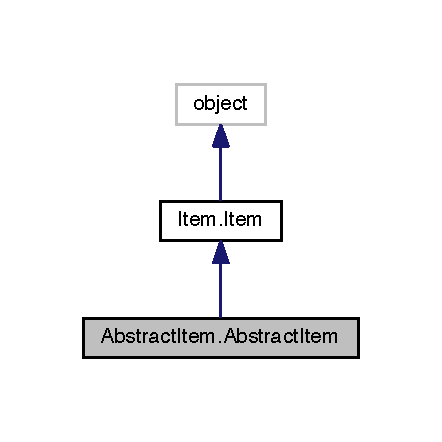
\includegraphics[width=212pt]{classAbstractItem_1_1AbstractItem__inherit__graph}
\end{center}
\end{figure}


Collaboration diagram for Abstract\+Item.\+Abstract\+Item\+:\nopagebreak
\begin{figure}[H]
\begin{center}
\leavevmode
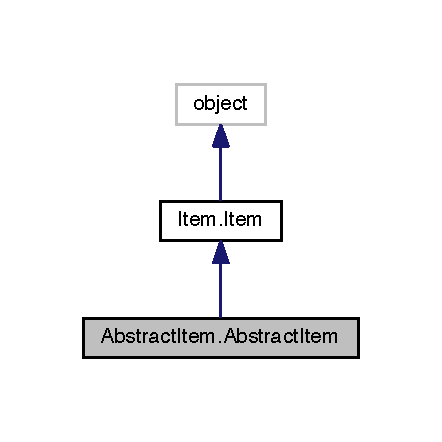
\includegraphics[width=212pt]{classAbstractItem_1_1AbstractItem__coll__graph}
\end{center}
\end{figure}
\subsection*{Public Member Functions}
\begin{DoxyCompactItemize}
\item 
def \hyperlink{classAbstractItem_1_1AbstractItem_a33578b09c4f0fd29c582bdd0e0977577}{\+\_\+\+\_\+init\+\_\+\+\_\+} (self, title, genre, barcode)
\begin{DoxyCompactList}\small\item\em Constructs a new \hyperlink{namespaceItem}{Item} with the given title, genre, and barcode. \end{DoxyCompactList}\item 
def \hyperlink{classAbstractItem_1_1AbstractItem_a566051dd4f0e9b3ba3ce8214a8779244}{is\+Rented} (self)
\begin{DoxyCompactList}\small\item\em Returns whether this item is rented. \end{DoxyCompactList}\item 
def \hyperlink{classAbstractItem_1_1AbstractItem_abcf92f11f8210ca0e413dc2bc64cb6aa}{get\+Due\+Date} (self)
\begin{DoxyCompactList}\small\item\em Returns this item due date. \end{DoxyCompactList}\item 
def \hyperlink{classAbstractItem_1_1AbstractItem_a9ab1907f5110c1047957f2d1f4bebb82}{get\+Title} (self)
\begin{DoxyCompactList}\small\item\em Returns this item title. \end{DoxyCompactList}\item 
def \hyperlink{classAbstractItem_1_1AbstractItem_a9c84bde2c7eadc30f70753b8c54b6fb3}{get\+Barcode} (self)
\begin{DoxyCompactList}\small\item\em Returns this item barcode. \end{DoxyCompactList}\item 
def \hyperlink{classAbstractItem_1_1AbstractItem_ac55364df8cb3e7a488842409c372d634}{\+\_\+\+\_\+str\+\_\+\+\_\+} (self)
\begin{DoxyCompactList}\small\item\em Returns a representation of the state of this object as a multiline string. \end{DoxyCompactList}\item 
def \hyperlink{classAbstractItem_1_1AbstractItem_aaa91fe39e01044fd43770867092d45ea}{\+\_\+\+\_\+eq\+\_\+\+\_\+} (self, obj)
\begin{DoxyCompactList}\small\item\em Determines whether this item is the same as another one based on its barcode. \end{DoxyCompactList}\end{DoxyCompactItemize}
\subsection*{Private Attributes}
\begin{DoxyCompactItemize}
\item 
\hyperlink{classAbstractItem_1_1AbstractItem_a2f4dc201ed6687e84b1b1b03863443c7}{\+\_\+\+\_\+title}
\begin{DoxyCompactList}\small\item\em Title of this item. \end{DoxyCompactList}\item 
\hyperlink{classAbstractItem_1_1AbstractItem_a9a18f410b1160da5c633a92ff228e5ee}{\+\_\+\+\_\+genre}
\begin{DoxyCompactList}\small\item\em Genre of this item. \end{DoxyCompactList}\item 
\hyperlink{classAbstractItem_1_1AbstractItem_a37fae73390cb431a6395a07ce5b5a5c7}{\+\_\+\+\_\+barcode}
\begin{DoxyCompactList}\small\item\em Unique Barcode for this item. \end{DoxyCompactList}\item 
\hyperlink{classAbstractItem_1_1AbstractItem_a5da9a42e491e8eb843fae960748ec7e7}{\+\_\+\+\_\+rented}
\begin{DoxyCompactList}\small\item\em Rental status of this item. \end{DoxyCompactList}\item 
\hyperlink{classAbstractItem_1_1AbstractItem_a6975f7e62b35b3162dd9c3aef089c1a3}{\+\_\+\+\_\+due\+Date}
\begin{DoxyCompactList}\small\item\em Due date for this item. \end{DoxyCompactList}\end{DoxyCompactItemize}


\subsection{Detailed Description}
Partial implementation of the \hyperlink{namespaceItem}{Item} interface. 

Definition at line 16 of file Abstract\+Item.\+py.



\subsection{Constructor \& Destructor Documentation}
\mbox{\Hypertarget{classAbstractItem_1_1AbstractItem_a33578b09c4f0fd29c582bdd0e0977577}\label{classAbstractItem_1_1AbstractItem_a33578b09c4f0fd29c582bdd0e0977577}} 
\index{Abstract\+Item\+::\+Abstract\+Item@{Abstract\+Item\+::\+Abstract\+Item}!\+\_\+\+\_\+init\+\_\+\+\_\+@{\+\_\+\+\_\+init\+\_\+\+\_\+}}
\index{\+\_\+\+\_\+init\+\_\+\+\_\+@{\+\_\+\+\_\+init\+\_\+\+\_\+}!Abstract\+Item\+::\+Abstract\+Item@{Abstract\+Item\+::\+Abstract\+Item}}
\subsubsection{\texorpdfstring{\+\_\+\+\_\+init\+\_\+\+\_\+()}{\_\_init\_\_()}}
{\footnotesize\ttfamily def Abstract\+Item.\+Abstract\+Item.\+\_\+\+\_\+init\+\_\+\+\_\+ (\begin{DoxyParamCaption}\item[{}]{self,  }\item[{}]{title,  }\item[{}]{genre,  }\item[{}]{barcode }\end{DoxyParamCaption})}



Constructs a new \hyperlink{namespaceItem}{Item} with the given title, genre, and barcode. 

This constructor may only be invoked by subclasses. 
\begin{DoxyParams}{Parameters}
{\em title} & the title of the item \\
\hline
{\em genre} & the genre of the item \\
\hline
{\em barcode} & a unique integer identifier for the item \\
\hline
\end{DoxyParams}


Definition at line 25 of file Abstract\+Item.\+py.



\subsection{Member Function Documentation}
\mbox{\Hypertarget{classAbstractItem_1_1AbstractItem_aaa91fe39e01044fd43770867092d45ea}\label{classAbstractItem_1_1AbstractItem_aaa91fe39e01044fd43770867092d45ea}} 
\index{Abstract\+Item\+::\+Abstract\+Item@{Abstract\+Item\+::\+Abstract\+Item}!\+\_\+\+\_\+eq\+\_\+\+\_\+@{\+\_\+\+\_\+eq\+\_\+\+\_\+}}
\index{\+\_\+\+\_\+eq\+\_\+\+\_\+@{\+\_\+\+\_\+eq\+\_\+\+\_\+}!Abstract\+Item\+::\+Abstract\+Item@{Abstract\+Item\+::\+Abstract\+Item}}
\subsubsection{\texorpdfstring{\+\_\+\+\_\+eq\+\_\+\+\_\+()}{\_\_eq\_\_()}}
{\footnotesize\ttfamily def Abstract\+Item.\+Abstract\+Item.\+\_\+\+\_\+eq\+\_\+\+\_\+ (\begin{DoxyParamCaption}\item[{}]{self,  }\item[{}]{obj }\end{DoxyParamCaption})}



Determines whether this item is the same as another one based on its barcode. 


\begin{DoxyParams}{Parameters}
{\em obj} & the object to compare to this item \\
\hline
\end{DoxyParams}
\begin{DoxyReturn}{Returns}
true if the given object is an \hyperlink{classAbstractItem_1_1AbstractItem}{Abstract\+Item} with the same barcode as this one 
\end{DoxyReturn}


Definition at line 95 of file Abstract\+Item.\+py.



References Abstract\+Item.\+Abstract\+Item.\+get\+Barcode().

\mbox{\Hypertarget{classAbstractItem_1_1AbstractItem_ac55364df8cb3e7a488842409c372d634}\label{classAbstractItem_1_1AbstractItem_ac55364df8cb3e7a488842409c372d634}} 
\index{Abstract\+Item\+::\+Abstract\+Item@{Abstract\+Item\+::\+Abstract\+Item}!\+\_\+\+\_\+str\+\_\+\+\_\+@{\+\_\+\+\_\+str\+\_\+\+\_\+}}
\index{\+\_\+\+\_\+str\+\_\+\+\_\+@{\+\_\+\+\_\+str\+\_\+\+\_\+}!Abstract\+Item\+::\+Abstract\+Item@{Abstract\+Item\+::\+Abstract\+Item}}
\subsubsection{\texorpdfstring{\+\_\+\+\_\+str\+\_\+\+\_\+()}{\_\_str\_\_()}}
{\footnotesize\ttfamily def Abstract\+Item.\+Abstract\+Item.\+\_\+\+\_\+str\+\_\+\+\_\+ (\begin{DoxyParamCaption}\item[{}]{self }\end{DoxyParamCaption})}



Returns a representation of the state of this object as a multiline string. 

The format is\+: 
\begin{DoxyPre}
    type
    title
    (genre)
    status
  \end{DoxyPre}
 The status is either 
\begin{DoxyPre}
    Rented: yyyy-mm-dd
  \end{DoxyPre}
 or 
\begin{DoxyPre}
    Available
  \end{DoxyPre}
 where \char`\"{}yyyy-\/mm-\/dd\char`\"{} is the current due date.

\begin{DoxyReturn}{Returns}
a string representation of this object 
\end{DoxyReturn}


Definition at line 76 of file Abstract\+Item.\+py.



References Abstract\+Item.\+Abstract\+Item.\+get\+Due\+Date(), Item.\+Item.\+get\+Genre(), Abstract\+Item.\+Abstract\+Item.\+get\+Title(), and Abstract\+Item.\+Abstract\+Item.\+is\+Rented().

\mbox{\Hypertarget{classAbstractItem_1_1AbstractItem_a9c84bde2c7eadc30f70753b8c54b6fb3}\label{classAbstractItem_1_1AbstractItem_a9c84bde2c7eadc30f70753b8c54b6fb3}} 
\index{Abstract\+Item\+::\+Abstract\+Item@{Abstract\+Item\+::\+Abstract\+Item}!get\+Barcode@{get\+Barcode}}
\index{get\+Barcode@{get\+Barcode}!Abstract\+Item\+::\+Abstract\+Item@{Abstract\+Item\+::\+Abstract\+Item}}
\subsubsection{\texorpdfstring{get\+Barcode()}{getBarcode()}}
{\footnotesize\ttfamily def Abstract\+Item.\+Abstract\+Item.\+get\+Barcode (\begin{DoxyParamCaption}\item[{}]{self }\end{DoxyParamCaption})}



Returns this item barcode. 



Definition at line 52 of file Abstract\+Item.\+py.



References Abstract\+Item.\+Abstract\+Item.\+\_\+\+\_\+barcode.



Referenced by Abstract\+Item.\+Abstract\+Item.\+\_\+\+\_\+eq\+\_\+\+\_\+().

\mbox{\Hypertarget{classAbstractItem_1_1AbstractItem_abcf92f11f8210ca0e413dc2bc64cb6aa}\label{classAbstractItem_1_1AbstractItem_abcf92f11f8210ca0e413dc2bc64cb6aa}} 
\index{Abstract\+Item\+::\+Abstract\+Item@{Abstract\+Item\+::\+Abstract\+Item}!get\+Due\+Date@{get\+Due\+Date}}
\index{get\+Due\+Date@{get\+Due\+Date}!Abstract\+Item\+::\+Abstract\+Item@{Abstract\+Item\+::\+Abstract\+Item}}
\subsubsection{\texorpdfstring{get\+Due\+Date()}{getDueDate()}}
{\footnotesize\ttfamily def Abstract\+Item.\+Abstract\+Item.\+get\+Due\+Date (\begin{DoxyParamCaption}\item[{}]{self }\end{DoxyParamCaption})}



Returns this item due date. 



Definition at line 42 of file Abstract\+Item.\+py.



References Abstract\+Item.\+Abstract\+Item.\+\_\+\+\_\+due\+Date.



Referenced by Abstract\+Item.\+Abstract\+Item.\+\_\+\+\_\+str\+\_\+\+\_\+().

\mbox{\Hypertarget{classAbstractItem_1_1AbstractItem_a9ab1907f5110c1047957f2d1f4bebb82}\label{classAbstractItem_1_1AbstractItem_a9ab1907f5110c1047957f2d1f4bebb82}} 
\index{Abstract\+Item\+::\+Abstract\+Item@{Abstract\+Item\+::\+Abstract\+Item}!get\+Title@{get\+Title}}
\index{get\+Title@{get\+Title}!Abstract\+Item\+::\+Abstract\+Item@{Abstract\+Item\+::\+Abstract\+Item}}
\subsubsection{\texorpdfstring{get\+Title()}{getTitle()}}
{\footnotesize\ttfamily def Abstract\+Item.\+Abstract\+Item.\+get\+Title (\begin{DoxyParamCaption}\item[{}]{self }\end{DoxyParamCaption})}



Returns this item title. 



Definition at line 48 of file Abstract\+Item.\+py.



References Abstract\+Item.\+Abstract\+Item.\+\_\+\+\_\+title.



Referenced by Abstract\+Item.\+Abstract\+Item.\+\_\+\+\_\+str\+\_\+\+\_\+().

\mbox{\Hypertarget{classAbstractItem_1_1AbstractItem_a566051dd4f0e9b3ba3ce8214a8779244}\label{classAbstractItem_1_1AbstractItem_a566051dd4f0e9b3ba3ce8214a8779244}} 
\index{Abstract\+Item\+::\+Abstract\+Item@{Abstract\+Item\+::\+Abstract\+Item}!is\+Rented@{is\+Rented}}
\index{is\+Rented@{is\+Rented}!Abstract\+Item\+::\+Abstract\+Item@{Abstract\+Item\+::\+Abstract\+Item}}
\subsubsection{\texorpdfstring{is\+Rented()}{isRented()}}
{\footnotesize\ttfamily def Abstract\+Item.\+Abstract\+Item.\+is\+Rented (\begin{DoxyParamCaption}\item[{}]{self }\end{DoxyParamCaption})}



Returns whether this item is rented. 



Definition at line 38 of file Abstract\+Item.\+py.



References Abstract\+Item.\+Abstract\+Item.\+\_\+\+\_\+rented.



Referenced by Abstract\+Item.\+Abstract\+Item.\+\_\+\+\_\+str\+\_\+\+\_\+().



\subsection{Member Data Documentation}
\mbox{\Hypertarget{classAbstractItem_1_1AbstractItem_a37fae73390cb431a6395a07ce5b5a5c7}\label{classAbstractItem_1_1AbstractItem_a37fae73390cb431a6395a07ce5b5a5c7}} 
\index{Abstract\+Item\+::\+Abstract\+Item@{Abstract\+Item\+::\+Abstract\+Item}!\+\_\+\+\_\+barcode@{\+\_\+\+\_\+barcode}}
\index{\+\_\+\+\_\+barcode@{\+\_\+\+\_\+barcode}!Abstract\+Item\+::\+Abstract\+Item@{Abstract\+Item\+::\+Abstract\+Item}}
\subsubsection{\texorpdfstring{\+\_\+\+\_\+barcode}{\_\_barcode}}
{\footnotesize\ttfamily Abstract\+Item.\+Abstract\+Item.\+\_\+\+\_\+barcode\hspace{0.3cm}{\ttfamily [private]}}



Unique Barcode for this item. 



Definition at line 31 of file Abstract\+Item.\+py.



Referenced by Abstract\+Item.\+Abstract\+Item.\+get\+Barcode().

\mbox{\Hypertarget{classAbstractItem_1_1AbstractItem_a6975f7e62b35b3162dd9c3aef089c1a3}\label{classAbstractItem_1_1AbstractItem_a6975f7e62b35b3162dd9c3aef089c1a3}} 
\index{Abstract\+Item\+::\+Abstract\+Item@{Abstract\+Item\+::\+Abstract\+Item}!\+\_\+\+\_\+due\+Date@{\+\_\+\+\_\+due\+Date}}
\index{\+\_\+\+\_\+due\+Date@{\+\_\+\+\_\+due\+Date}!Abstract\+Item\+::\+Abstract\+Item@{Abstract\+Item\+::\+Abstract\+Item}}
\subsubsection{\texorpdfstring{\+\_\+\+\_\+due\+Date}{\_\_dueDate}}
{\footnotesize\ttfamily Abstract\+Item.\+Abstract\+Item.\+\_\+\+\_\+due\+Date\hspace{0.3cm}{\ttfamily [private]}}



Due date for this item. 



Definition at line 35 of file Abstract\+Item.\+py.



Referenced by Abstract\+Item.\+Abstract\+Item.\+get\+Due\+Date().

\mbox{\Hypertarget{classAbstractItem_1_1AbstractItem_a9a18f410b1160da5c633a92ff228e5ee}\label{classAbstractItem_1_1AbstractItem_a9a18f410b1160da5c633a92ff228e5ee}} 
\index{Abstract\+Item\+::\+Abstract\+Item@{Abstract\+Item\+::\+Abstract\+Item}!\+\_\+\+\_\+genre@{\+\_\+\+\_\+genre}}
\index{\+\_\+\+\_\+genre@{\+\_\+\+\_\+genre}!Abstract\+Item\+::\+Abstract\+Item@{Abstract\+Item\+::\+Abstract\+Item}}
\subsubsection{\texorpdfstring{\+\_\+\+\_\+genre}{\_\_genre}}
{\footnotesize\ttfamily Abstract\+Item.\+Abstract\+Item.\+\_\+\+\_\+genre\hspace{0.3cm}{\ttfamily [private]}}



Genre of this item. 



Definition at line 29 of file Abstract\+Item.\+py.



Referenced by Genre\+Search.\+Genre\+Search.\+matches().

\mbox{\Hypertarget{classAbstractItem_1_1AbstractItem_a5da9a42e491e8eb843fae960748ec7e7}\label{classAbstractItem_1_1AbstractItem_a5da9a42e491e8eb843fae960748ec7e7}} 
\index{Abstract\+Item\+::\+Abstract\+Item@{Abstract\+Item\+::\+Abstract\+Item}!\+\_\+\+\_\+rented@{\+\_\+\+\_\+rented}}
\index{\+\_\+\+\_\+rented@{\+\_\+\+\_\+rented}!Abstract\+Item\+::\+Abstract\+Item@{Abstract\+Item\+::\+Abstract\+Item}}
\subsubsection{\texorpdfstring{\+\_\+\+\_\+rented}{\_\_rented}}
{\footnotesize\ttfamily Abstract\+Item.\+Abstract\+Item.\+\_\+\+\_\+rented\hspace{0.3cm}{\ttfamily [private]}}



Rental status of this item. 



Definition at line 33 of file Abstract\+Item.\+py.



Referenced by Abstract\+Item.\+Abstract\+Item.\+is\+Rented().

\mbox{\Hypertarget{classAbstractItem_1_1AbstractItem_a2f4dc201ed6687e84b1b1b03863443c7}\label{classAbstractItem_1_1AbstractItem_a2f4dc201ed6687e84b1b1b03863443c7}} 
\index{Abstract\+Item\+::\+Abstract\+Item@{Abstract\+Item\+::\+Abstract\+Item}!\+\_\+\+\_\+title@{\+\_\+\+\_\+title}}
\index{\+\_\+\+\_\+title@{\+\_\+\+\_\+title}!Abstract\+Item\+::\+Abstract\+Item@{Abstract\+Item\+::\+Abstract\+Item}}
\subsubsection{\texorpdfstring{\+\_\+\+\_\+title}{\_\_title}}
{\footnotesize\ttfamily Abstract\+Item.\+Abstract\+Item.\+\_\+\+\_\+title\hspace{0.3cm}{\ttfamily [private]}}



Title of this item. 



Definition at line 27 of file Abstract\+Item.\+py.



Referenced by Abstract\+Item.\+Abstract\+Item.\+get\+Title().



The documentation for this class was generated from the following file\+:\begin{DoxyCompactItemize}
\item 
\hyperlink{AbstractItem_8py}{Abstract\+Item.\+py}\end{DoxyCompactItemize}

\hypertarget{classCustomer_1_1Customer}{}\section{Customer.\+Customer Class Reference}
\label{classCustomer_1_1Customer}\index{Customer.\+Customer@{Customer.\+Customer}}


A \hyperlink{classCustomer_1_1Customer}{Customer} is a client of a \hyperlink{namespaceVideoStore}{Video\+Store} who can rent items.  


\subsection*{Public Member Functions}
\begin{DoxyCompactItemize}
\item 
def \hyperlink{classCustomer_1_1Customer_a9a6e72f7972ab6669244ee32b5c15fa8}{\+\_\+\+\_\+init\+\_\+\+\_\+} (self, name)
\begin{DoxyCompactList}\small\item\em Constructs a \hyperlink{classCustomer_1_1Customer}{Customer} with the given name. \end{DoxyCompactList}\item 
def \hyperlink{classCustomer_1_1Customer_aeda8ba0748ed02a22582207d04d90d62}{rent\+Item} (self, item, today)
\begin{DoxyCompactList}\small\item\em Rents an item and adds it to this customer\textquotesingle{}s list of items. \end{DoxyCompactList}\item 
def \hyperlink{classCustomer_1_1Customer_ac589f3f34db4ca44e3071e7260f5f8b6}{bring\+Back\+Item} (self, barcode, today)
\begin{DoxyCompactList}\small\item\em Returns an item that this customer currently has rented and updates the balance if a late fee or credit is due. \end{DoxyCompactList}\item 
def \hyperlink{classCustomer_1_1Customer_aebb56585524424bcededa48f90a2dde6}{get\+Balance} (self)
\begin{DoxyCompactList}\small\item\em Returns the balance for this customer. \end{DoxyCompactList}\item 
def \hyperlink{classCustomer_1_1Customer_a154e1dbfb02e85d29b52e620b6283677}{get\+Name} (self)
\begin{DoxyCompactList}\small\item\em Returns the name of this customer. \end{DoxyCompactList}\item 
def \hyperlink{classCustomer_1_1Customer_a87070bd1a552dd094365dc4464253a3a}{make\+Payment} (self, amount)
\begin{DoxyCompactList}\small\item\em Makes a payment on this customer\textquotesingle{}s balance. \end{DoxyCompactList}\item 
def \hyperlink{classCustomer_1_1Customer_aa12655d57338586f1ee2a5c101d44356}{\+\_\+\+\_\+str\+\_\+\+\_\+} (self)
\begin{DoxyCompactList}\small\item\em Returns a string representation of this customer. \end{DoxyCompactList}\item 
def \hyperlink{classCustomer_1_1Customer_ad2f1246cd764010c5701930f6576f5e0}{can\+Rent} (self, today)
\begin{DoxyCompactList}\small\item\em Helper method determines whether this customer already has overdue items. \end{DoxyCompactList}\end{DoxyCompactItemize}
\subsection*{Private Attributes}
\begin{DoxyCompactItemize}
\item 
\hyperlink{classCustomer_1_1Customer_a573f55a71c994b6881a99fe055e9e1c2}{\+\_\+\+\_\+items\+Out}
\begin{DoxyCompactList}\small\item\em Items currently rented by this customer. \end{DoxyCompactList}\item 
\hyperlink{classCustomer_1_1Customer_a400a0ef109352dbf3f843006f22e611f}{\+\_\+\+\_\+name}
\begin{DoxyCompactList}\small\item\em Name of this customer. \end{DoxyCompactList}\item 
\hyperlink{classCustomer_1_1Customer_a3fe2716ffce15422d3bebc6989a1353d}{\+\_\+\+\_\+balance}
\begin{DoxyCompactList}\small\item\em Balance currently owed by this customer. \end{DoxyCompactList}\end{DoxyCompactItemize}


\subsection{Detailed Description}
A \hyperlink{classCustomer_1_1Customer}{Customer} is a client of a \hyperlink{namespaceVideoStore}{Video\+Store} who can rent items. 

A client is identified by a unique name. At any given time a \hyperlink{classCustomer_1_1Customer}{Customer} has a list of items currently rented, and a balance representing rental charges, late fees, or credits (where a negative balance indicates a credit). Balances are in cents. Ordinary customers are not allowed to rent new items if they have any items overdue. 

Definition at line 25 of file Customer.\+py.



\subsection{Constructor \& Destructor Documentation}
\mbox{\Hypertarget{classCustomer_1_1Customer_a9a6e72f7972ab6669244ee32b5c15fa8}\label{classCustomer_1_1Customer_a9a6e72f7972ab6669244ee32b5c15fa8}} 
\index{Customer\+::\+Customer@{Customer\+::\+Customer}!\+\_\+\+\_\+init\+\_\+\+\_\+@{\+\_\+\+\_\+init\+\_\+\+\_\+}}
\index{\+\_\+\+\_\+init\+\_\+\+\_\+@{\+\_\+\+\_\+init\+\_\+\+\_\+}!Customer\+::\+Customer@{Customer\+::\+Customer}}
\subsubsection{\texorpdfstring{\+\_\+\+\_\+init\+\_\+\+\_\+()}{\_\_init\_\_()}}
{\footnotesize\ttfamily def Customer.\+Customer.\+\_\+\+\_\+init\+\_\+\+\_\+ (\begin{DoxyParamCaption}\item[{}]{self,  }\item[{}]{name }\end{DoxyParamCaption})}



Constructs a \hyperlink{classCustomer_1_1Customer}{Customer} with the given name. 

Initially there are no items rented and the balance is zero. 
\begin{DoxyParams}{Parameters}
{\em name} & the new customer\textquotesingle{}s name \\
\hline
\end{DoxyParams}


Definition at line 33 of file Customer.\+py.



\subsection{Member Function Documentation}
\mbox{\Hypertarget{classCustomer_1_1Customer_aa12655d57338586f1ee2a5c101d44356}\label{classCustomer_1_1Customer_aa12655d57338586f1ee2a5c101d44356}} 
\index{Customer\+::\+Customer@{Customer\+::\+Customer}!\+\_\+\+\_\+str\+\_\+\+\_\+@{\+\_\+\+\_\+str\+\_\+\+\_\+}}
\index{\+\_\+\+\_\+str\+\_\+\+\_\+@{\+\_\+\+\_\+str\+\_\+\+\_\+}!Customer\+::\+Customer@{Customer\+::\+Customer}}
\subsubsection{\texorpdfstring{\+\_\+\+\_\+str\+\_\+\+\_\+()}{\_\_str\_\_()}}
{\footnotesize\ttfamily def Customer.\+Customer.\+\_\+\+\_\+str\+\_\+\+\_\+ (\begin{DoxyParamCaption}\item[{}]{self }\end{DoxyParamCaption})}



Returns a string representation of this customer. 

The format consists of multiple lines. The first line is the patron\textquotesingle{}s name. Subsequent lines are formed from the {\bfseries str}() values of the items currently rented, separated by a newline. \begin{DoxyReturn}{Returns}
representation of this object as a multi-\/line string 
\end{DoxyReturn}


Definition at line 110 of file Customer.\+py.



References Customer.\+Customer.\+\_\+\+\_\+items\+Out, and Customer.\+Customer.\+\_\+\+\_\+name.

\mbox{\Hypertarget{classCustomer_1_1Customer_ac589f3f34db4ca44e3071e7260f5f8b6}\label{classCustomer_1_1Customer_ac589f3f34db4ca44e3071e7260f5f8b6}} 
\index{Customer\+::\+Customer@{Customer\+::\+Customer}!bring\+Back\+Item@{bring\+Back\+Item}}
\index{bring\+Back\+Item@{bring\+Back\+Item}!Customer\+::\+Customer@{Customer\+::\+Customer}}
\subsubsection{\texorpdfstring{bring\+Back\+Item()}{bringBackItem()}}
{\footnotesize\ttfamily def Customer.\+Customer.\+bring\+Back\+Item (\begin{DoxyParamCaption}\item[{}]{self,  }\item[{}]{barcode,  }\item[{}]{today }\end{DoxyParamCaption})}



Returns an item that this customer currently has rented and updates the balance if a late fee or credit is due. 

If the item can be successfully returned, this method updates the item\textquotesingle{}s status and removes it from this customer\textquotesingle{}s list of items. If the customer does not have the item rented, a \hyperlink{namespaceStatusException}{Status\+Exception} is thrown. 
\begin{DoxyParams}{Parameters}
{\em barcode} & identifier for the item to be returned \\
\hline
{\em today} & the date on which the item is being returned \\
\hline
\end{DoxyParams}

\begin{DoxyExceptions}{Exceptions}
{\em \hyperlink{namespaceStatusException}{Status\+Exception}} & if this customer does not have the given item rented \\
\hline
\end{DoxyExceptions}


Definition at line 73 of file Customer.\+py.

\mbox{\Hypertarget{classCustomer_1_1Customer_ad2f1246cd764010c5701930f6576f5e0}\label{classCustomer_1_1Customer_ad2f1246cd764010c5701930f6576f5e0}} 
\index{Customer\+::\+Customer@{Customer\+::\+Customer}!can\+Rent@{can\+Rent}}
\index{can\+Rent@{can\+Rent}!Customer\+::\+Customer@{Customer\+::\+Customer}}
\subsubsection{\texorpdfstring{can\+Rent()}{canRent()}}
{\footnotesize\ttfamily def Customer.\+Customer.\+can\+Rent (\begin{DoxyParamCaption}\item[{}]{self,  }\item[{}]{today }\end{DoxyParamCaption})}



Helper method determines whether this customer already has overdue items. 


\begin{DoxyParams}{Parameters}
{\em today} & the current date \\
\hline
\end{DoxyParams}
\begin{DoxyReturn}{Returns}
true if the customer has no overdue items, false otherwise 
\end{DoxyReturn}


Definition at line 126 of file Customer.\+py.



References Customer.\+Customer.\+\_\+\+\_\+items\+Out.



Referenced by Customer.\+Customer.\+rent\+Item().

\mbox{\Hypertarget{classCustomer_1_1Customer_aebb56585524424bcededa48f90a2dde6}\label{classCustomer_1_1Customer_aebb56585524424bcededa48f90a2dde6}} 
\index{Customer\+::\+Customer@{Customer\+::\+Customer}!get\+Balance@{get\+Balance}}
\index{get\+Balance@{get\+Balance}!Customer\+::\+Customer@{Customer\+::\+Customer}}
\subsubsection{\texorpdfstring{get\+Balance()}{getBalance()}}
{\footnotesize\ttfamily def Customer.\+Customer.\+get\+Balance (\begin{DoxyParamCaption}\item[{}]{self }\end{DoxyParamCaption})}



Returns the balance for this customer. 

\begin{DoxyReturn}{Returns}
this customer\textquotesingle{}s balance 
\end{DoxyReturn}


Definition at line 83 of file Customer.\+py.



References Customer.\+Customer.\+\_\+\+\_\+balance.

\mbox{\Hypertarget{classCustomer_1_1Customer_a154e1dbfb02e85d29b52e620b6283677}\label{classCustomer_1_1Customer_a154e1dbfb02e85d29b52e620b6283677}} 
\index{Customer\+::\+Customer@{Customer\+::\+Customer}!get\+Name@{get\+Name}}
\index{get\+Name@{get\+Name}!Customer\+::\+Customer@{Customer\+::\+Customer}}
\subsubsection{\texorpdfstring{get\+Name()}{getName()}}
{\footnotesize\ttfamily def Customer.\+Customer.\+get\+Name (\begin{DoxyParamCaption}\item[{}]{self }\end{DoxyParamCaption})}



Returns the name of this customer. 

\begin{DoxyReturn}{Returns}
this customer\textquotesingle{}s name 
\end{DoxyReturn}


Definition at line 91 of file Customer.\+py.



References Customer.\+Customer.\+\_\+\+\_\+name.

\mbox{\Hypertarget{classCustomer_1_1Customer_a87070bd1a552dd094365dc4464253a3a}\label{classCustomer_1_1Customer_a87070bd1a552dd094365dc4464253a3a}} 
\index{Customer\+::\+Customer@{Customer\+::\+Customer}!make\+Payment@{make\+Payment}}
\index{make\+Payment@{make\+Payment}!Customer\+::\+Customer@{Customer\+::\+Customer}}
\subsubsection{\texorpdfstring{make\+Payment()}{makePayment()}}
{\footnotesize\ttfamily def Customer.\+Customer.\+make\+Payment (\begin{DoxyParamCaption}\item[{}]{self,  }\item[{}]{amount }\end{DoxyParamCaption})}



Makes a payment on this customer\textquotesingle{}s balance. 


\begin{DoxyParams}{Parameters}
{\em amount} & the amount to be paid, in cents \\
\hline
\end{DoxyParams}


Definition at line 99 of file Customer.\+py.



References Customer.\+Customer.\+\_\+\+\_\+balance.

\mbox{\Hypertarget{classCustomer_1_1Customer_aeda8ba0748ed02a22582207d04d90d62}\label{classCustomer_1_1Customer_aeda8ba0748ed02a22582207d04d90d62}} 
\index{Customer\+::\+Customer@{Customer\+::\+Customer}!rent\+Item@{rent\+Item}}
\index{rent\+Item@{rent\+Item}!Customer\+::\+Customer@{Customer\+::\+Customer}}
\subsubsection{\texorpdfstring{rent\+Item()}{rentItem()}}
{\footnotesize\ttfamily def Customer.\+Customer.\+rent\+Item (\begin{DoxyParamCaption}\item[{}]{self,  }\item[{}]{item,  }\item[{}]{today }\end{DoxyParamCaption})}



Rents an item and adds it to this customer\textquotesingle{}s list of items. 

If the item can be rented, this method updates the item\textquotesingle{}s status (including the due date) and then adds it to this customer\textquotesingle{}s list of items. If the item cannot be rented to this customer, a \hyperlink{namespaceStatusException}{Status\+Exception} is thrown. 
\begin{DoxyParams}{Parameters}
{\em item} & the item to be rented \\
\hline
{\em today} & the date on which the item is being rented \\
\hline
\end{DoxyParams}

\begin{DoxyExceptions}{Exceptions}
{\em \hyperlink{namespaceStatusException}{Status\+Exception}} & if the item cannot be rented to this customer for any reason \\
\hline
\end{DoxyExceptions}


Definition at line 53 of file Customer.\+py.



References Customer.\+Customer.\+\_\+\+\_\+balance, Customer.\+Customer.\+\_\+\+\_\+items\+Out, and Customer.\+Customer.\+can\+Rent().



\subsection{Member Data Documentation}
\mbox{\Hypertarget{classCustomer_1_1Customer_a3fe2716ffce15422d3bebc6989a1353d}\label{classCustomer_1_1Customer_a3fe2716ffce15422d3bebc6989a1353d}} 
\index{Customer\+::\+Customer@{Customer\+::\+Customer}!\+\_\+\+\_\+balance@{\+\_\+\+\_\+balance}}
\index{\+\_\+\+\_\+balance@{\+\_\+\+\_\+balance}!Customer\+::\+Customer@{Customer\+::\+Customer}}
\subsubsection{\texorpdfstring{\+\_\+\+\_\+balance}{\_\_balance}}
{\footnotesize\ttfamily Customer.\+Customer.\+\_\+\+\_\+balance\hspace{0.3cm}{\ttfamily [private]}}



Balance currently owed by this customer. 



Definition at line 39 of file Customer.\+py.



Referenced by Customer.\+Customer.\+get\+Balance(), Customer.\+Customer.\+make\+Payment(), and Customer.\+Customer.\+rent\+Item().

\mbox{\Hypertarget{classCustomer_1_1Customer_a573f55a71c994b6881a99fe055e9e1c2}\label{classCustomer_1_1Customer_a573f55a71c994b6881a99fe055e9e1c2}} 
\index{Customer\+::\+Customer@{Customer\+::\+Customer}!\+\_\+\+\_\+items\+Out@{\+\_\+\+\_\+items\+Out}}
\index{\+\_\+\+\_\+items\+Out@{\+\_\+\+\_\+items\+Out}!Customer\+::\+Customer@{Customer\+::\+Customer}}
\subsubsection{\texorpdfstring{\+\_\+\+\_\+items\+Out}{\_\_itemsOut}}
{\footnotesize\ttfamily Customer.\+Customer.\+\_\+\+\_\+items\+Out\hspace{0.3cm}{\ttfamily [private]}}



Items currently rented by this customer. 



Definition at line 35 of file Customer.\+py.



Referenced by Customer.\+Customer.\+\_\+\+\_\+str\+\_\+\+\_\+(), Customer.\+Customer.\+can\+Rent(), and Customer.\+Customer.\+rent\+Item().

\mbox{\Hypertarget{classCustomer_1_1Customer_a400a0ef109352dbf3f843006f22e611f}\label{classCustomer_1_1Customer_a400a0ef109352dbf3f843006f22e611f}} 
\index{Customer\+::\+Customer@{Customer\+::\+Customer}!\+\_\+\+\_\+name@{\+\_\+\+\_\+name}}
\index{\+\_\+\+\_\+name@{\+\_\+\+\_\+name}!Customer\+::\+Customer@{Customer\+::\+Customer}}
\subsubsection{\texorpdfstring{\+\_\+\+\_\+name}{\_\_name}}
{\footnotesize\ttfamily Customer.\+Customer.\+\_\+\+\_\+name\hspace{0.3cm}{\ttfamily [private]}}



Name of this customer. 



Definition at line 37 of file Customer.\+py.



Referenced by Customer.\+Customer.\+\_\+\+\_\+str\+\_\+\+\_\+(), and Customer.\+Customer.\+get\+Name().



The documentation for this class was generated from the following file\+:\begin{DoxyCompactItemize}
\item 
\hyperlink{Customer_8py}{Customer.\+py}\end{DoxyCompactItemize}

\hypertarget{classGenreSearch_1_1GenreSearch}{}\section{Genre\+Search.\+Genre\+Search Class Reference}
\label{classGenreSearch_1_1GenreSearch}\index{Genre\+Search.\+Genre\+Search@{Genre\+Search.\+Genre\+Search}}


Implementation of \hyperlink{namespaceSearchCondition}{Search\+Condition} that matches items based on the genre (not case sensitive).  




Inheritance diagram for Genre\+Search.\+Genre\+Search\+:\nopagebreak
\begin{figure}[H]
\begin{center}
\leavevmode
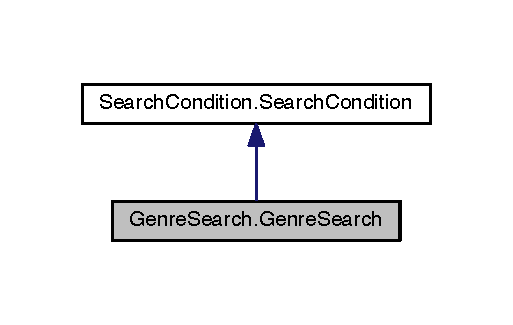
\includegraphics[width=246pt]{classGenreSearch_1_1GenreSearch__inherit__graph}
\end{center}
\end{figure}


Collaboration diagram for Genre\+Search.\+Genre\+Search\+:\nopagebreak
\begin{figure}[H]
\begin{center}
\leavevmode
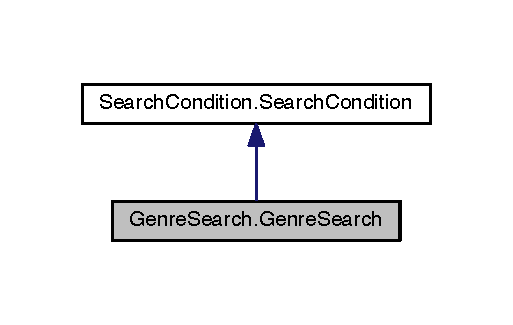
\includegraphics[width=246pt]{classGenreSearch_1_1GenreSearch__coll__graph}
\end{center}
\end{figure}
\subsection*{Public Member Functions}
\begin{DoxyCompactItemize}
\item 
def \hyperlink{classGenreSearch_1_1GenreSearch_ad098e5ccc44530bafd752eca9b928ea7}{\+\_\+\+\_\+init\+\_\+\+\_\+} (self, genre)
\begin{DoxyCompactList}\small\item\em Constructs a \hyperlink{classGenreSearch_1_1GenreSearch}{Genre\+Search} for the given value. \end{DoxyCompactList}\item 
def \hyperlink{classGenreSearch_1_1GenreSearch_a5804ebb42a3d38e89a4591be173a22d0}{matches} (self, item)
\begin{DoxyCompactList}\small\item\em Matches this genre with the genre of a given item. \end{DoxyCompactList}\end{DoxyCompactItemize}
\subsection*{Private Attributes}
\begin{DoxyCompactItemize}
\item 
\hyperlink{classGenreSearch_1_1GenreSearch_a659affb5b3425cb942692d18a3d47b36}{\+\_\+\+\_\+genre}
\begin{DoxyCompactList}\small\item\em The genre we are searching for. \end{DoxyCompactList}\end{DoxyCompactItemize}


\subsection{Detailed Description}
Implementation of \hyperlink{namespaceSearchCondition}{Search\+Condition} that matches items based on the genre (not case sensitive). 

Definition at line 17 of file Genre\+Search.\+py.



\subsection{Constructor \& Destructor Documentation}
\mbox{\Hypertarget{classGenreSearch_1_1GenreSearch_ad098e5ccc44530bafd752eca9b928ea7}\label{classGenreSearch_1_1GenreSearch_ad098e5ccc44530bafd752eca9b928ea7}} 
\index{Genre\+Search\+::\+Genre\+Search@{Genre\+Search\+::\+Genre\+Search}!\+\_\+\+\_\+init\+\_\+\+\_\+@{\+\_\+\+\_\+init\+\_\+\+\_\+}}
\index{\+\_\+\+\_\+init\+\_\+\+\_\+@{\+\_\+\+\_\+init\+\_\+\+\_\+}!Genre\+Search\+::\+Genre\+Search@{Genre\+Search\+::\+Genre\+Search}}
\subsubsection{\texorpdfstring{\+\_\+\+\_\+init\+\_\+\+\_\+()}{\_\_init\_\_()}}
{\footnotesize\ttfamily def Genre\+Search.\+Genre\+Search.\+\_\+\+\_\+init\+\_\+\+\_\+ (\begin{DoxyParamCaption}\item[{}]{self,  }\item[{}]{genre }\end{DoxyParamCaption})}



Constructs a \hyperlink{classGenreSearch_1_1GenreSearch}{Genre\+Search} for the given value. 


\begin{DoxyParams}{Parameters}
{\em genre} & the genre to search for \\
\hline
\end{DoxyParams}


Definition at line 24 of file Genre\+Search.\+py.



\subsection{Member Function Documentation}
\mbox{\Hypertarget{classGenreSearch_1_1GenreSearch_a5804ebb42a3d38e89a4591be173a22d0}\label{classGenreSearch_1_1GenreSearch_a5804ebb42a3d38e89a4591be173a22d0}} 
\index{Genre\+Search\+::\+Genre\+Search@{Genre\+Search\+::\+Genre\+Search}!matches@{matches}}
\index{matches@{matches}!Genre\+Search\+::\+Genre\+Search@{Genre\+Search\+::\+Genre\+Search}}
\subsubsection{\texorpdfstring{matches()}{matches()}}
{\footnotesize\ttfamily def Genre\+Search.\+Genre\+Search.\+matches (\begin{DoxyParamCaption}\item[{}]{self,  }\item[{}]{item }\end{DoxyParamCaption})}



Matches this genre with the genre of a given item. 


\begin{DoxyParams}{Parameters}
{\em item} & containing the genre to compare to. \\
\hline
\end{DoxyParams}


Definition at line 33 of file Genre\+Search.\+py.



References Genre\+Search.\+Genre\+Search.\+\_\+\+\_\+genre, and Abstract\+Item.\+Abstract\+Item.\+\_\+\+\_\+genre.



\subsection{Member Data Documentation}
\mbox{\Hypertarget{classGenreSearch_1_1GenreSearch_a659affb5b3425cb942692d18a3d47b36}\label{classGenreSearch_1_1GenreSearch_a659affb5b3425cb942692d18a3d47b36}} 
\index{Genre\+Search\+::\+Genre\+Search@{Genre\+Search\+::\+Genre\+Search}!\+\_\+\+\_\+genre@{\+\_\+\+\_\+genre}}
\index{\+\_\+\+\_\+genre@{\+\_\+\+\_\+genre}!Genre\+Search\+::\+Genre\+Search@{Genre\+Search\+::\+Genre\+Search}}
\subsubsection{\texorpdfstring{\+\_\+\+\_\+genre}{\_\_genre}}
{\footnotesize\ttfamily Genre\+Search.\+Genre\+Search.\+\_\+\+\_\+genre\hspace{0.3cm}{\ttfamily [private]}}



The genre we are searching for. 



Definition at line 26 of file Genre\+Search.\+py.



Referenced by Genre\+Search.\+Genre\+Search.\+matches().



The documentation for this class was generated from the following file\+:\begin{DoxyCompactItemize}
\item 
\hyperlink{GenreSearch_8py}{Genre\+Search.\+py}\end{DoxyCompactItemize}

\hypertarget{classItem_1_1Item}{}\section{Item.\+Item Class Reference}
\label{classItem_1_1Item}\index{Item.\+Item@{Item.\+Item}}


This is an abstract class.  




Inheritance diagram for Item.\+Item\+:\nopagebreak
\begin{figure}[H]
\begin{center}
\leavevmode
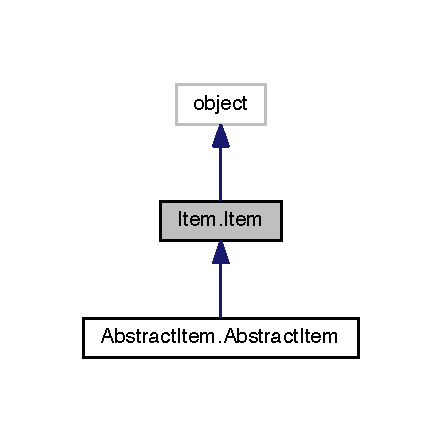
\includegraphics[width=212pt]{classItem_1_1Item__inherit__graph}
\end{center}
\end{figure}


Collaboration diagram for Item.\+Item\+:\nopagebreak
\begin{figure}[H]
\begin{center}
\leavevmode
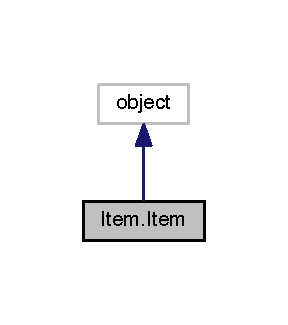
\includegraphics[width=138pt]{classItem_1_1Item__coll__graph}
\end{center}
\end{figure}
\subsection*{Public Member Functions}
\begin{DoxyCompactItemize}
\item 
def \hyperlink{classItem_1_1Item_a866dd05fa3e3ab124f6afeaa171ab516}{set\+Rented} (self, today)
\begin{DoxyCompactList}\small\item\em Rents this item if it is not already rented and sets the due date. \end{DoxyCompactList}\item 
def \hyperlink{classItem_1_1Item_afc0dccd77c3d32664c5a424886d7d53c}{set\+Returned} (self, today)
\begin{DoxyCompactList}\small\item\em Returns this item, if it is currently rented. \end{DoxyCompactList}\item 
def \hyperlink{classItem_1_1Item_afe4448d1a099b956ecc0fc66ca22925d}{get\+Rental\+Cost} (self)
\begin{DoxyCompactList}\small\item\em Returns the cost to rent this item. \end{DoxyCompactList}\item 
def \hyperlink{classItem_1_1Item_a17d1bdd2d1f6d4ad81a9d1fd0b2d149d}{calculate\+Late\+Fee} (self, today)
\begin{DoxyCompactList}\small\item\em Calculates the late fee (or bonus) that would be charged (or applied) for returning the item on the given date. \end{DoxyCompactList}\item 
def \hyperlink{classItem_1_1Item_a4f815eee80b9dffbbc0be9d79a0520ff}{get\+Genre} (self)
\begin{DoxyCompactList}\small\item\em Returns a String representing the genre of this item. \end{DoxyCompactList}\item 
def \hyperlink{classItem_1_1Item_a2dcb80d5765c07aefe735cd657385764}{is\+Rented} (self)
\begin{DoxyCompactList}\small\item\em Determines whether this item is currently rented. \end{DoxyCompactList}\item 
def \hyperlink{classItem_1_1Item_a14c6c86e71412609102c9fb0cd009751}{get\+Due\+Date} (self)
\begin{DoxyCompactList}\small\item\em Returns the due date for this item if it is currently rented, or null if the item is not rented. \end{DoxyCompactList}\item 
def \hyperlink{classItem_1_1Item_a2b359025258f0b0f0ef33d7da4f806fa}{get\+Title} (self)
\begin{DoxyCompactList}\small\item\em Returns the title of this item. \end{DoxyCompactList}\item 
def \hyperlink{classItem_1_1Item_ac53c971f8932eb428ee5a9999ba8c541}{get\+Barcode} (self)
\begin{DoxyCompactList}\small\item\em Returns the integer barcode for this item. \end{DoxyCompactList}\end{DoxyCompactItemize}


\subsection{Detailed Description}
This is an abstract class. 

All methods here must be implemented elsewhere.

An item represents a movie or game that can be rented from a video store. Each item has a title, a genre, and a unique integer identifier called a barcode. An item can be rented or available, and if rented it has a due date. 

Definition at line 21 of file Item.\+py.



\subsection{Member Function Documentation}
\mbox{\Hypertarget{classItem_1_1Item_a17d1bdd2d1f6d4ad81a9d1fd0b2d149d}\label{classItem_1_1Item_a17d1bdd2d1f6d4ad81a9d1fd0b2d149d}} 
\index{Item\+::\+Item@{Item\+::\+Item}!calculate\+Late\+Fee@{calculate\+Late\+Fee}}
\index{calculate\+Late\+Fee@{calculate\+Late\+Fee}!Item\+::\+Item@{Item\+::\+Item}}
\subsubsection{\texorpdfstring{calculate\+Late\+Fee()}{calculateLateFee()}}
{\footnotesize\ttfamily def Item.\+Item.\+calculate\+Late\+Fee (\begin{DoxyParamCaption}\item[{}]{self,  }\item[{}]{today }\end{DoxyParamCaption})}



Calculates the late fee (or bonus) that would be charged (or applied) for returning the item on the given date. 


\begin{DoxyParams}{Parameters}
{\em today} & the date on which the item is being returned \\
\hline
\end{DoxyParams}
\begin{DoxyReturn}{Returns}
the late fee or bonus for returning the item on the given date, or zero if the item is not currently rented 
\end{DoxyReturn}


Definition at line 60 of file Item.\+py.

\mbox{\Hypertarget{classItem_1_1Item_ac53c971f8932eb428ee5a9999ba8c541}\label{classItem_1_1Item_ac53c971f8932eb428ee5a9999ba8c541}} 
\index{Item\+::\+Item@{Item\+::\+Item}!get\+Barcode@{get\+Barcode}}
\index{get\+Barcode@{get\+Barcode}!Item\+::\+Item@{Item\+::\+Item}}
\subsubsection{\texorpdfstring{get\+Barcode()}{getBarcode()}}
{\footnotesize\ttfamily def Item.\+Item.\+get\+Barcode (\begin{DoxyParamCaption}\item[{}]{self }\end{DoxyParamCaption})}



Returns the integer barcode for this item. 

\begin{DoxyReturn}{Returns}
barcode of this item 
\end{DoxyReturn}


Definition at line 101 of file Item.\+py.

\mbox{\Hypertarget{classItem_1_1Item_a14c6c86e71412609102c9fb0cd009751}\label{classItem_1_1Item_a14c6c86e71412609102c9fb0cd009751}} 
\index{Item\+::\+Item@{Item\+::\+Item}!get\+Due\+Date@{get\+Due\+Date}}
\index{get\+Due\+Date@{get\+Due\+Date}!Item\+::\+Item@{Item\+::\+Item}}
\subsubsection{\texorpdfstring{get\+Due\+Date()}{getDueDate()}}
{\footnotesize\ttfamily def Item.\+Item.\+get\+Due\+Date (\begin{DoxyParamCaption}\item[{}]{self }\end{DoxyParamCaption})}



Returns the due date for this item if it is currently rented, or null if the item is not rented. 

\begin{DoxyReturn}{Returns}
due date for this item 
\end{DoxyReturn}


Definition at line 85 of file Item.\+py.

\mbox{\Hypertarget{classItem_1_1Item_a4f815eee80b9dffbbc0be9d79a0520ff}\label{classItem_1_1Item_a4f815eee80b9dffbbc0be9d79a0520ff}} 
\index{Item\+::\+Item@{Item\+::\+Item}!get\+Genre@{get\+Genre}}
\index{get\+Genre@{get\+Genre}!Item\+::\+Item@{Item\+::\+Item}}
\subsubsection{\texorpdfstring{get\+Genre()}{getGenre()}}
{\footnotesize\ttfamily def Item.\+Item.\+get\+Genre (\begin{DoxyParamCaption}\item[{}]{self }\end{DoxyParamCaption})}



Returns a String representing the genre of this item. 

\begin{DoxyReturn}{Returns}
genre of this item 
\end{DoxyReturn}


Definition at line 68 of file Item.\+py.



Referenced by Abstract\+Item.\+Abstract\+Item.\+\_\+\+\_\+str\+\_\+\+\_\+().

\mbox{\Hypertarget{classItem_1_1Item_afe4448d1a099b956ecc0fc66ca22925d}\label{classItem_1_1Item_afe4448d1a099b956ecc0fc66ca22925d}} 
\index{Item\+::\+Item@{Item\+::\+Item}!get\+Rental\+Cost@{get\+Rental\+Cost}}
\index{get\+Rental\+Cost@{get\+Rental\+Cost}!Item\+::\+Item@{Item\+::\+Item}}
\subsubsection{\texorpdfstring{get\+Rental\+Cost()}{getRentalCost()}}
{\footnotesize\ttfamily def Item.\+Item.\+get\+Rental\+Cost (\begin{DoxyParamCaption}\item[{}]{self }\end{DoxyParamCaption})}



Returns the cost to rent this item. 

\begin{DoxyReturn}{Returns}
cost to rent the item 
\end{DoxyReturn}


Definition at line 48 of file Item.\+py.

\mbox{\Hypertarget{classItem_1_1Item_a2b359025258f0b0f0ef33d7da4f806fa}\label{classItem_1_1Item_a2b359025258f0b0f0ef33d7da4f806fa}} 
\index{Item\+::\+Item@{Item\+::\+Item}!get\+Title@{get\+Title}}
\index{get\+Title@{get\+Title}!Item\+::\+Item@{Item\+::\+Item}}
\subsubsection{\texorpdfstring{get\+Title()}{getTitle()}}
{\footnotesize\ttfamily def Item.\+Item.\+get\+Title (\begin{DoxyParamCaption}\item[{}]{self }\end{DoxyParamCaption})}



Returns the title of this item. 

\begin{DoxyReturn}{Returns}
title of this item 
\end{DoxyReturn}


Definition at line 93 of file Item.\+py.

\mbox{\Hypertarget{classItem_1_1Item_a2dcb80d5765c07aefe735cd657385764}\label{classItem_1_1Item_a2dcb80d5765c07aefe735cd657385764}} 
\index{Item\+::\+Item@{Item\+::\+Item}!is\+Rented@{is\+Rented}}
\index{is\+Rented@{is\+Rented}!Item\+::\+Item@{Item\+::\+Item}}
\subsubsection{\texorpdfstring{is\+Rented()}{isRented()}}
{\footnotesize\ttfamily def Item.\+Item.\+is\+Rented (\begin{DoxyParamCaption}\item[{}]{self }\end{DoxyParamCaption})}



Determines whether this item is currently rented. 

\begin{DoxyReturn}{Returns}
true if this item is rented, false otherwise 
\end{DoxyReturn}


Definition at line 76 of file Item.\+py.

\mbox{\Hypertarget{classItem_1_1Item_a866dd05fa3e3ab124f6afeaa171ab516}\label{classItem_1_1Item_a866dd05fa3e3ab124f6afeaa171ab516}} 
\index{Item\+::\+Item@{Item\+::\+Item}!set\+Rented@{set\+Rented}}
\index{set\+Rented@{set\+Rented}!Item\+::\+Item@{Item\+::\+Item}}
\subsubsection{\texorpdfstring{set\+Rented()}{setRented()}}
{\footnotesize\ttfamily def Item.\+Item.\+set\+Rented (\begin{DoxyParamCaption}\item[{}]{self,  }\item[{}]{today }\end{DoxyParamCaption})}



Rents this item if it is not already rented and sets the due date. 


\begin{DoxyParams}{Parameters}
{\em today} & the date on which this item is being rented \\
\hline
\end{DoxyParams}

\begin{DoxyExceptions}{Exceptions}
{\em \hyperlink{namespaceStatusException}{Status\+Exception}} & if the item cannot be rented \\
\hline
\end{DoxyExceptions}


Definition at line 30 of file Item.\+py.

\mbox{\Hypertarget{classItem_1_1Item_afc0dccd77c3d32664c5a424886d7d53c}\label{classItem_1_1Item_afc0dccd77c3d32664c5a424886d7d53c}} 
\index{Item\+::\+Item@{Item\+::\+Item}!set\+Returned@{set\+Returned}}
\index{set\+Returned@{set\+Returned}!Item\+::\+Item@{Item\+::\+Item}}
\subsubsection{\texorpdfstring{set\+Returned()}{setReturned()}}
{\footnotesize\ttfamily def Item.\+Item.\+set\+Returned (\begin{DoxyParamCaption}\item[{}]{self,  }\item[{}]{today }\end{DoxyParamCaption})}



Returns this item, if it is currently rented. 


\begin{DoxyParams}{Parameters}
{\em today} & the date on which the item is being returned \\
\hline
\end{DoxyParams}

\begin{DoxyExceptions}{Exceptions}
{\em \hyperlink{namespaceStatusException}{Status\+Exception}} & if the item is not currently rented \\
\hline
\end{DoxyExceptions}


Definition at line 40 of file Item.\+py.



The documentation for this class was generated from the following file\+:\begin{DoxyCompactItemize}
\item 
\hyperlink{Item_8py}{Item.\+py}\end{DoxyCompactItemize}

\hypertarget{classSearchCondition_1_1SearchCondition}{}\section{Search\+Condition.\+Search\+Condition Class Reference}
\label{classSearchCondition_1_1SearchCondition}\index{Search\+Condition.\+Search\+Condition@{Search\+Condition.\+Search\+Condition}}


Abstraction of a search predicate for items.  




Inheritance diagram for Search\+Condition.\+Search\+Condition\+:\nopagebreak
\begin{figure}[H]
\begin{center}
\leavevmode
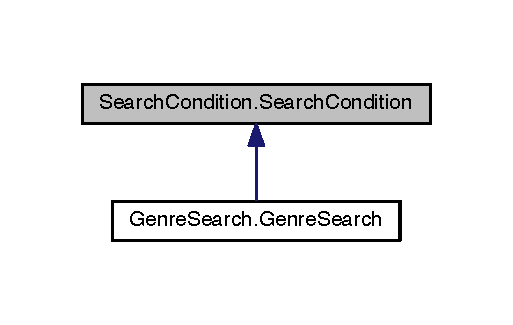
\includegraphics[width=246pt]{classSearchCondition_1_1SearchCondition__inherit__graph}
\end{center}
\end{figure}
\subsection*{Public Member Functions}
\begin{DoxyCompactItemize}
\item 
def \hyperlink{classSearchCondition_1_1SearchCondition_a3e1b1fe7a20c9b86a8716a756bb3849c}{matches} (self, item)
\begin{DoxyCompactList}\small\item\em Determine whether the given item matches this search condition\textquotesingle{}s criteria for inclusion. \end{DoxyCompactList}\end{DoxyCompactItemize}


\subsection{Detailed Description}
Abstraction of a search predicate for items. 

Subtypes can customize the nature of the search (e.\+g., exact title, title keywords, genre, etc.). 

Definition at line 16 of file Search\+Condition.\+py.



\subsection{Member Function Documentation}
\mbox{\Hypertarget{classSearchCondition_1_1SearchCondition_a3e1b1fe7a20c9b86a8716a756bb3849c}\label{classSearchCondition_1_1SearchCondition_a3e1b1fe7a20c9b86a8716a756bb3849c}} 
\index{Search\+Condition\+::\+Search\+Condition@{Search\+Condition\+::\+Search\+Condition}!matches@{matches}}
\index{matches@{matches}!Search\+Condition\+::\+Search\+Condition@{Search\+Condition\+::\+Search\+Condition}}
\subsubsection{\texorpdfstring{matches()}{matches()}}
{\footnotesize\ttfamily def Search\+Condition.\+Search\+Condition.\+matches (\begin{DoxyParamCaption}\item[{}]{self,  }\item[{}]{item }\end{DoxyParamCaption})}



Determine whether the given item matches this search condition\textquotesingle{}s criteria for inclusion. 


\begin{DoxyParams}{Parameters}
{\em item} & the item to be checked \\
\hline
\end{DoxyParams}
\begin{DoxyReturn}{Returns}
true if the item matches this condition\textquotesingle{}s criteria, false otherwise 
\end{DoxyReturn}


Definition at line 24 of file Search\+Condition.\+py.



The documentation for this class was generated from the following file\+:\begin{DoxyCompactItemize}
\item 
\hyperlink{SearchCondition_8py}{Search\+Condition.\+py}\end{DoxyCompactItemize}

\hypertarget{classSimpleDate_1_1SimpleDate}{}\section{Simple\+Date.\+Simple\+Date Class Reference}
\label{classSimpleDate_1_1SimpleDate}\index{Simple\+Date.\+Simple\+Date@{Simple\+Date.\+Simple\+Date}}


Date consisting of a year, month, and day.  


\subsection*{Public Member Functions}
\begin{DoxyCompactItemize}
\item 
def \hyperlink{classSimpleDate_1_1SimpleDate_a8e01278f5e3987e64396ef345ccb7dde}{\+\_\+\+\_\+init\+\_\+\+\_\+} (self, year, month, day)
\begin{DoxyCompactList}\small\item\em Constructs a \hyperlink{classSimpleDate_1_1SimpleDate}{Simple\+Date} with the given year, month, and day. \end{DoxyCompactList}\item 
def \hyperlink{classSimpleDate_1_1SimpleDate_a84c11740813035133e89c4f55d35268d}{Simple\+Date\+From\+Days} (self, existing, additional\+Days)
\begin{DoxyCompactList}\small\item\em Returns a \hyperlink{classSimpleDate_1_1SimpleDate}{Simple\+Date} that is a given number of days after an existing date. \end{DoxyCompactList}\item 
def \hyperlink{classSimpleDate_1_1SimpleDate_a3f991d5bf914be8175808732a37296c4}{is\+Before} (self, other)
\begin{DoxyCompactList}\small\item\em Determines whether this date is strictly earlier than the given date. \end{DoxyCompactList}\item 
def \hyperlink{classSimpleDate_1_1SimpleDate_a9e6a7a4fa0751c99c28dc7130c849944}{days\+Until} (self, other)
\begin{DoxyCompactList}\small\item\em Returns the number of days from this date until the given date. \end{DoxyCompactList}\item 
def \hyperlink{classSimpleDate_1_1SimpleDate_ad33dd54a78befede77ffed77c85d6861}{\+\_\+\+\_\+str\+\_\+\+\_\+} (self)
\begin{DoxyCompactList}\small\item\em Prints this simple\+Date in the format year-\/month-\/day. \end{DoxyCompactList}\end{DoxyCompactItemize}
\subsection*{Static Public Attributes}
\begin{DoxyCompactItemize}
\item 
int \hyperlink{classSimpleDate_1_1SimpleDate_a0481c6d110c7475177a3e59aa89fb20b}{M\+I\+L\+L\+I\+S\+\_\+\+I\+N\+\_\+24\+\_\+\+H\+O\+U\+RS} = 1000 $\ast$ 60 $\ast$ 60 $\ast$ 24
\begin{DoxyCompactList}\small\item\em Number of millisecons in one day. \end{DoxyCompactList}\end{DoxyCompactItemize}
\subsection*{Private Attributes}
\begin{DoxyCompactItemize}
\item 
\hyperlink{classSimpleDate_1_1SimpleDate_a0ae516370c49819c39e89606e163a875}{\+\_\+\+\_\+date}
\begin{DoxyCompactList}\small\item\em Holds the date in this \hyperlink{classSimpleDate_1_1SimpleDate}{Simple\+Date} object. \end{DoxyCompactList}\end{DoxyCompactItemize}


\subsection{Detailed Description}
Date consisting of a year, month, and day. 

Definition at line 16 of file Simple\+Date.\+py.



\subsection{Constructor \& Destructor Documentation}
\mbox{\Hypertarget{classSimpleDate_1_1SimpleDate_a8e01278f5e3987e64396ef345ccb7dde}\label{classSimpleDate_1_1SimpleDate_a8e01278f5e3987e64396ef345ccb7dde}} 
\index{Simple\+Date\+::\+Simple\+Date@{Simple\+Date\+::\+Simple\+Date}!\+\_\+\+\_\+init\+\_\+\+\_\+@{\+\_\+\+\_\+init\+\_\+\+\_\+}}
\index{\+\_\+\+\_\+init\+\_\+\+\_\+@{\+\_\+\+\_\+init\+\_\+\+\_\+}!Simple\+Date\+::\+Simple\+Date@{Simple\+Date\+::\+Simple\+Date}}
\subsubsection{\texorpdfstring{\+\_\+\+\_\+init\+\_\+\+\_\+()}{\_\_init\_\_()}}
{\footnotesize\ttfamily def Simple\+Date.\+Simple\+Date.\+\_\+\+\_\+init\+\_\+\+\_\+ (\begin{DoxyParamCaption}\item[{}]{self,  }\item[{}]{year,  }\item[{}]{month,  }\item[{}]{day }\end{DoxyParamCaption})}



Constructs a \hyperlink{classSimpleDate_1_1SimpleDate}{Simple\+Date} with the given year, month, and day. 


\begin{DoxyParams}{Parameters}
{\em year} & four-\/digit year \\
\hline
{\em month} & 1-\/based month number \\
\hline
{\em day} & 1-\/based day of month \\
\hline
\end{DoxyParams}


Definition at line 27 of file Simple\+Date.\+py.



\subsection{Member Function Documentation}
\mbox{\Hypertarget{classSimpleDate_1_1SimpleDate_ad33dd54a78befede77ffed77c85d6861}\label{classSimpleDate_1_1SimpleDate_ad33dd54a78befede77ffed77c85d6861}} 
\index{Simple\+Date\+::\+Simple\+Date@{Simple\+Date\+::\+Simple\+Date}!\+\_\+\+\_\+str\+\_\+\+\_\+@{\+\_\+\+\_\+str\+\_\+\+\_\+}}
\index{\+\_\+\+\_\+str\+\_\+\+\_\+@{\+\_\+\+\_\+str\+\_\+\+\_\+}!Simple\+Date\+::\+Simple\+Date@{Simple\+Date\+::\+Simple\+Date}}
\subsubsection{\texorpdfstring{\+\_\+\+\_\+str\+\_\+\+\_\+()}{\_\_str\_\_()}}
{\footnotesize\ttfamily def Simple\+Date.\+Simple\+Date.\+\_\+\+\_\+str\+\_\+\+\_\+ (\begin{DoxyParamCaption}\item[{}]{self }\end{DoxyParamCaption})}



Prints this simple\+Date in the format year-\/month-\/day. 



Definition at line 66 of file Simple\+Date.\+py.



References Simple\+Date.\+Simple\+Date.\+\_\+\+\_\+date.

\mbox{\Hypertarget{classSimpleDate_1_1SimpleDate_a9e6a7a4fa0751c99c28dc7130c849944}\label{classSimpleDate_1_1SimpleDate_a9e6a7a4fa0751c99c28dc7130c849944}} 
\index{Simple\+Date\+::\+Simple\+Date@{Simple\+Date\+::\+Simple\+Date}!days\+Until@{days\+Until}}
\index{days\+Until@{days\+Until}!Simple\+Date\+::\+Simple\+Date@{Simple\+Date\+::\+Simple\+Date}}
\subsubsection{\texorpdfstring{days\+Until()}{daysUntil()}}
{\footnotesize\ttfamily def Simple\+Date.\+Simple\+Date.\+days\+Until (\begin{DoxyParamCaption}\item[{}]{self,  }\item[{}]{other }\end{DoxyParamCaption})}



Returns the number of days from this date until the given date. 

Returns a negative number if this date after the given date. 
\begin{DoxyParams}{Parameters}
{\em other} & the future date \\
\hline
\end{DoxyParams}
\begin{DoxyReturn}{Returns}
number of days until the given date (negative if it is in the past) 
\end{DoxyReturn}


Definition at line 60 of file Simple\+Date.\+py.



References Simple\+Date.\+Simple\+Date.\+\_\+\+\_\+date.



Referenced by Simple\+Date.\+Simple\+Date.\+is\+Before().

\mbox{\Hypertarget{classSimpleDate_1_1SimpleDate_a3f991d5bf914be8175808732a37296c4}\label{classSimpleDate_1_1SimpleDate_a3f991d5bf914be8175808732a37296c4}} 
\index{Simple\+Date\+::\+Simple\+Date@{Simple\+Date\+::\+Simple\+Date}!is\+Before@{is\+Before}}
\index{is\+Before@{is\+Before}!Simple\+Date\+::\+Simple\+Date@{Simple\+Date\+::\+Simple\+Date}}
\subsubsection{\texorpdfstring{is\+Before()}{isBefore()}}
{\footnotesize\ttfamily def Simple\+Date.\+Simple\+Date.\+is\+Before (\begin{DoxyParamCaption}\item[{}]{self,  }\item[{}]{other }\end{DoxyParamCaption})}



Determines whether this date is strictly earlier than the given date. 


\begin{DoxyParams}{Parameters}
{\em other} & \\
\hline
\end{DoxyParams}
\begin{DoxyReturn}{Returns}
true if this date is strictly before the given date. false otherwise 
\end{DoxyReturn}


Definition at line 51 of file Simple\+Date.\+py.



References Simple\+Date.\+Simple\+Date.\+days\+Until().

\mbox{\Hypertarget{classSimpleDate_1_1SimpleDate_a84c11740813035133e89c4f55d35268d}\label{classSimpleDate_1_1SimpleDate_a84c11740813035133e89c4f55d35268d}} 
\index{Simple\+Date\+::\+Simple\+Date@{Simple\+Date\+::\+Simple\+Date}!Simple\+Date\+From\+Days@{Simple\+Date\+From\+Days}}
\index{Simple\+Date\+From\+Days@{Simple\+Date\+From\+Days}!Simple\+Date\+::\+Simple\+Date@{Simple\+Date\+::\+Simple\+Date}}
\subsubsection{\texorpdfstring{Simple\+Date\+From\+Days()}{SimpleDateFromDays()}}
{\footnotesize\ttfamily def Simple\+Date.\+Simple\+Date.\+Simple\+Date\+From\+Days (\begin{DoxyParamCaption}\item[{}]{self,  }\item[{}]{existing,  }\item[{}]{additional\+Days }\end{DoxyParamCaption})}



Returns a \hyperlink{classSimpleDate_1_1SimpleDate}{Simple\+Date} that is a given number of days after an existing date. 


\begin{DoxyParams}{Parameters}
{\em existing} & the given \hyperlink{classSimpleDate_1_1SimpleDate}{Simple\+Date} \\
\hline
{\em additional\+Days} & the number of days to be added to the existing date \\
\hline
\end{DoxyParams}


Definition at line 38 of file Simple\+Date.\+py.



\subsection{Member Data Documentation}
\mbox{\Hypertarget{classSimpleDate_1_1SimpleDate_a0ae516370c49819c39e89606e163a875}\label{classSimpleDate_1_1SimpleDate_a0ae516370c49819c39e89606e163a875}} 
\index{Simple\+Date\+::\+Simple\+Date@{Simple\+Date\+::\+Simple\+Date}!\+\_\+\+\_\+date@{\+\_\+\+\_\+date}}
\index{\+\_\+\+\_\+date@{\+\_\+\+\_\+date}!Simple\+Date\+::\+Simple\+Date@{Simple\+Date\+::\+Simple\+Date}}
\subsubsection{\texorpdfstring{\+\_\+\+\_\+date}{\_\_date}}
{\footnotesize\ttfamily Simple\+Date.\+Simple\+Date.\+\_\+\+\_\+date\hspace{0.3cm}{\ttfamily [private]}}



Holds the date in this \hyperlink{classSimpleDate_1_1SimpleDate}{Simple\+Date} object. 



Definition at line 30 of file Simple\+Date.\+py.



Referenced by Simple\+Date.\+Simple\+Date.\+\_\+\+\_\+str\+\_\+\+\_\+(), and Simple\+Date.\+Simple\+Date.\+days\+Until().

\mbox{\Hypertarget{classSimpleDate_1_1SimpleDate_a0481c6d110c7475177a3e59aa89fb20b}\label{classSimpleDate_1_1SimpleDate_a0481c6d110c7475177a3e59aa89fb20b}} 
\index{Simple\+Date\+::\+Simple\+Date@{Simple\+Date\+::\+Simple\+Date}!M\+I\+L\+L\+I\+S\+\_\+\+I\+N\+\_\+24\+\_\+\+H\+O\+U\+RS@{M\+I\+L\+L\+I\+S\+\_\+\+I\+N\+\_\+24\+\_\+\+H\+O\+U\+RS}}
\index{M\+I\+L\+L\+I\+S\+\_\+\+I\+N\+\_\+24\+\_\+\+H\+O\+U\+RS@{M\+I\+L\+L\+I\+S\+\_\+\+I\+N\+\_\+24\+\_\+\+H\+O\+U\+RS}!Simple\+Date\+::\+Simple\+Date@{Simple\+Date\+::\+Simple\+Date}}
\subsubsection{\texorpdfstring{M\+I\+L\+L\+I\+S\+\_\+\+I\+N\+\_\+24\+\_\+\+H\+O\+U\+RS}{MILLIS\_IN\_24\_HOURS}}
{\footnotesize\ttfamily int Simple\+Date.\+Simple\+Date.\+M\+I\+L\+L\+I\+S\+\_\+\+I\+N\+\_\+24\+\_\+\+H\+O\+U\+RS = 1000 $\ast$ 60 $\ast$ 60 $\ast$ 24\hspace{0.3cm}{\ttfamily [static]}}



Number of millisecons in one day. 



Definition at line 19 of file Simple\+Date.\+py.



The documentation for this class was generated from the following file\+:\begin{DoxyCompactItemize}
\item 
\hyperlink{SimpleDate_8py}{Simple\+Date.\+py}\end{DoxyCompactItemize}

\hypertarget{classStatusException_1_1StatusException}{}\section{Status\+Exception.\+Status\+Exception Class Reference}
\label{classStatusException_1_1StatusException}\index{Status\+Exception.\+Status\+Exception@{Status\+Exception.\+Status\+Exception}}


Exception type thrown for invalid operations such as attempting to rent an item that is already rented.  




Inheritance diagram for Status\+Exception.\+Status\+Exception\+:\nopagebreak
\begin{figure}[H]
\begin{center}
\leavevmode
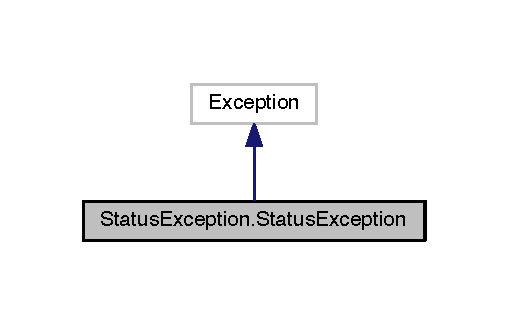
\includegraphics[width=244pt]{classStatusException_1_1StatusException__inherit__graph}
\end{center}
\end{figure}


Collaboration diagram for Status\+Exception.\+Status\+Exception\+:\nopagebreak
\begin{figure}[H]
\begin{center}
\leavevmode
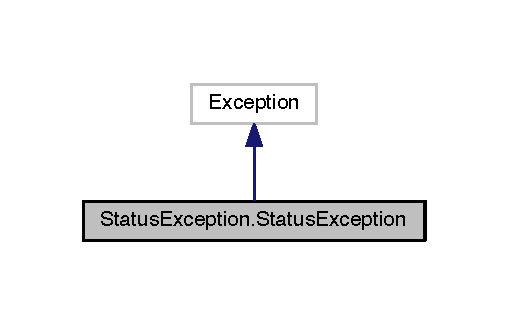
\includegraphics[width=244pt]{classStatusException_1_1StatusException__coll__graph}
\end{center}
\end{figure}
\subsection*{Public Member Functions}
\begin{DoxyCompactItemize}
\item 
def \hyperlink{classStatusException_1_1StatusException_a2b3f98decbd77f5e59626b9b50b27a36}{\+\_\+\+\_\+init\+\_\+\+\_\+} (self, \hyperlink{classStatusException_1_1StatusException_a4f3ffa4a96ccf5ca673e9e800d2f4c56}{msg})
\begin{DoxyCompactList}\small\item\em Constructs a \hyperlink{classStatusException_1_1StatusException}{Status\+Exception} with the given message. \end{DoxyCompactList}\end{DoxyCompactItemize}
\subsection*{Public Attributes}
\begin{DoxyCompactItemize}
\item 
\hyperlink{classStatusException_1_1StatusException_a4f3ffa4a96ccf5ca673e9e800d2f4c56}{msg}
\begin{DoxyCompactList}\small\item\em hold the error message. \end{DoxyCompactList}\end{DoxyCompactItemize}


\subsection{Detailed Description}
Exception type thrown for invalid operations such as attempting to rent an item that is already rented. 

Definition at line 16 of file Status\+Exception.\+py.



\subsection{Constructor \& Destructor Documentation}
\mbox{\Hypertarget{classStatusException_1_1StatusException_a2b3f98decbd77f5e59626b9b50b27a36}\label{classStatusException_1_1StatusException_a2b3f98decbd77f5e59626b9b50b27a36}} 
\index{Status\+Exception\+::\+Status\+Exception@{Status\+Exception\+::\+Status\+Exception}!\+\_\+\+\_\+init\+\_\+\+\_\+@{\+\_\+\+\_\+init\+\_\+\+\_\+}}
\index{\+\_\+\+\_\+init\+\_\+\+\_\+@{\+\_\+\+\_\+init\+\_\+\+\_\+}!Status\+Exception\+::\+Status\+Exception@{Status\+Exception\+::\+Status\+Exception}}
\subsubsection{\texorpdfstring{\+\_\+\+\_\+init\+\_\+\+\_\+()}{\_\_init\_\_()}}
{\footnotesize\ttfamily def Status\+Exception.\+Status\+Exception.\+\_\+\+\_\+init\+\_\+\+\_\+ (\begin{DoxyParamCaption}\item[{}]{self,  }\item[{}]{msg }\end{DoxyParamCaption})}



Constructs a \hyperlink{classStatusException_1_1StatusException}{Status\+Exception} with the given message. 


\begin{DoxyParams}{Parameters}
{\em msg} & message for this exception \\
\hline
\end{DoxyParams}


Definition at line 22 of file Status\+Exception.\+py.



\subsection{Member Data Documentation}
\mbox{\Hypertarget{classStatusException_1_1StatusException_a4f3ffa4a96ccf5ca673e9e800d2f4c56}\label{classStatusException_1_1StatusException_a4f3ffa4a96ccf5ca673e9e800d2f4c56}} 
\index{Status\+Exception\+::\+Status\+Exception@{Status\+Exception\+::\+Status\+Exception}!msg@{msg}}
\index{msg@{msg}!Status\+Exception\+::\+Status\+Exception@{Status\+Exception\+::\+Status\+Exception}}
\subsubsection{\texorpdfstring{msg}{msg}}
{\footnotesize\ttfamily Status\+Exception.\+Status\+Exception.\+msg}



hold the error message. 



Definition at line 26 of file Status\+Exception.\+py.



The documentation for this class was generated from the following file\+:\begin{DoxyCompactItemize}
\item 
\hyperlink{StatusException_8py}{Status\+Exception.\+py}\end{DoxyCompactItemize}

\hypertarget{classVideoStore_1_1VideoStore}{}\section{Video\+Store.\+Video\+Store Class Reference}
\label{classVideoStore_1_1VideoStore}\index{Video\+Store.\+Video\+Store@{Video\+Store.\+Video\+Store}}


\hyperlink{classVideoStore_1_1VideoStore}{Video\+Store} consists of a list of items and a list of customers who can rent items.  


\subsection*{Public Member Functions}
\begin{DoxyCompactItemize}
\item 
def \hyperlink{classVideoStore_1_1VideoStore_ae5c993cbfde1d6a6b872471dd8113184}{\+\_\+\+\_\+init\+\_\+\+\_\+} (self)
\begin{DoxyCompactList}\small\item\em Constructs a \hyperlink{classVideoStore_1_1VideoStore}{Video\+Store} that initially has no items and no customers. \end{DoxyCompactList}\item 
def \hyperlink{classVideoStore_1_1VideoStore_ad34e486af714a9513bff371d77b5dbbf}{add\+Item} (self, item)
\begin{DoxyCompactList}\small\item\em Adds an item to this store\textquotesingle{}s list of items, provided that there is not already an item with the same barcode. \end{DoxyCompactList}\item 
def \hyperlink{classVideoStore_1_1VideoStore_a9580d5be76ce527ceef595dc600ff92c}{add\+Customer} (self, customer)
\begin{DoxyCompactList}\small\item\em Adds a customer to this store\textquotesingle{}s list of customers. \end{DoxyCompactList}\item 
def \hyperlink{classVideoStore_1_1VideoStore_a864a5c88322cc7fe8d469963af6fbb74}{find\+User} (self, name)
\begin{DoxyCompactList}\small\item\em Returns the customer with the given name. \end{DoxyCompactList}\item 
def \hyperlink{classVideoStore_1_1VideoStore_a29c4c5fb82ee840192af398692d41cf3}{search} (self, condition)
\begin{DoxyCompactList}\small\item\em Search the store\textquotesingle{}s collection of for items satisfying the given \hyperlink{namespaceSearchCondition}{Search\+Condition}. \end{DoxyCompactList}\item 
def \hyperlink{classVideoStore_1_1VideoStore_a3c4bdb8e1df76ed65d00fdb32da18a3c}{\+\_\+\+\_\+str\+\_\+\+\_\+} (self)
\begin{DoxyCompactList}\small\item\em Returns the set of users and items in this store. \end{DoxyCompactList}\end{DoxyCompactItemize}
\subsection*{Private Attributes}
\begin{DoxyCompactItemize}
\item 
\hyperlink{classVideoStore_1_1VideoStore_a9b95fd49486fc2730c11920059fa1786}{\+\_\+\+\_\+items}
\begin{DoxyCompactList}\small\item\em The items in this store. \end{DoxyCompactList}\item 
\hyperlink{classVideoStore_1_1VideoStore_ab8f773ef96cc4f8aca5b845d9c32da0e}{\+\_\+\+\_\+customers}
\begin{DoxyCompactList}\small\item\em The list of customers of this store. \end{DoxyCompactList}\end{DoxyCompactItemize}


\subsection{Detailed Description}
\hyperlink{classVideoStore_1_1VideoStore}{Video\+Store} consists of a list of items and a list of customers who can rent items. 

Definition at line 20 of file Video\+Store.\+py.



\subsection{Constructor \& Destructor Documentation}
\mbox{\Hypertarget{classVideoStore_1_1VideoStore_ae5c993cbfde1d6a6b872471dd8113184}\label{classVideoStore_1_1VideoStore_ae5c993cbfde1d6a6b872471dd8113184}} 
\index{Video\+Store\+::\+Video\+Store@{Video\+Store\+::\+Video\+Store}!\+\_\+\+\_\+init\+\_\+\+\_\+@{\+\_\+\+\_\+init\+\_\+\+\_\+}}
\index{\+\_\+\+\_\+init\+\_\+\+\_\+@{\+\_\+\+\_\+init\+\_\+\+\_\+}!Video\+Store\+::\+Video\+Store@{Video\+Store\+::\+Video\+Store}}
\subsubsection{\texorpdfstring{\+\_\+\+\_\+init\+\_\+\+\_\+()}{\_\_init\_\_()}}
{\footnotesize\ttfamily def Video\+Store.\+Video\+Store.\+\_\+\+\_\+init\+\_\+\+\_\+ (\begin{DoxyParamCaption}\item[{}]{self }\end{DoxyParamCaption})}



Constructs a \hyperlink{classVideoStore_1_1VideoStore}{Video\+Store} that initially has no items and no customers. 



Definition at line 25 of file Video\+Store.\+py.



\subsection{Member Function Documentation}
\mbox{\Hypertarget{classVideoStore_1_1VideoStore_a3c4bdb8e1df76ed65d00fdb32da18a3c}\label{classVideoStore_1_1VideoStore_a3c4bdb8e1df76ed65d00fdb32da18a3c}} 
\index{Video\+Store\+::\+Video\+Store@{Video\+Store\+::\+Video\+Store}!\+\_\+\+\_\+str\+\_\+\+\_\+@{\+\_\+\+\_\+str\+\_\+\+\_\+}}
\index{\+\_\+\+\_\+str\+\_\+\+\_\+@{\+\_\+\+\_\+str\+\_\+\+\_\+}!Video\+Store\+::\+Video\+Store@{Video\+Store\+::\+Video\+Store}}
\subsubsection{\texorpdfstring{\+\_\+\+\_\+str\+\_\+\+\_\+()}{\_\_str\_\_()}}
{\footnotesize\ttfamily def Video\+Store.\+Video\+Store.\+\_\+\+\_\+str\+\_\+\+\_\+ (\begin{DoxyParamCaption}\item[{}]{self }\end{DoxyParamCaption})}



Returns the set of users and items in this store. 

\begin{DoxyReturn}{Returns}
a string with all users and items. 
\end{DoxyReturn}


Definition at line 81 of file Video\+Store.\+py.



References Video\+Store.\+Video\+Store.\+\_\+\+\_\+customers, and Video\+Store.\+Video\+Store.\+\_\+\+\_\+items.

\mbox{\Hypertarget{classVideoStore_1_1VideoStore_a9580d5be76ce527ceef595dc600ff92c}\label{classVideoStore_1_1VideoStore_a9580d5be76ce527ceef595dc600ff92c}} 
\index{Video\+Store\+::\+Video\+Store@{Video\+Store\+::\+Video\+Store}!add\+Customer@{add\+Customer}}
\index{add\+Customer@{add\+Customer}!Video\+Store\+::\+Video\+Store@{Video\+Store\+::\+Video\+Store}}
\subsubsection{\texorpdfstring{add\+Customer()}{addCustomer()}}
{\footnotesize\ttfamily def Video\+Store.\+Video\+Store.\+add\+Customer (\begin{DoxyParamCaption}\item[{}]{self,  }\item[{}]{customer }\end{DoxyParamCaption})}



Adds a customer to this store\textquotesingle{}s list of customers. 


\begin{DoxyParams}{Parameters}
{\em customer} & the customer to be added \\
\hline
\end{DoxyParams}


Definition at line 45 of file Video\+Store.\+py.



References Video\+Store.\+Video\+Store.\+\_\+\+\_\+customers.

\mbox{\Hypertarget{classVideoStore_1_1VideoStore_ad34e486af714a9513bff371d77b5dbbf}\label{classVideoStore_1_1VideoStore_ad34e486af714a9513bff371d77b5dbbf}} 
\index{Video\+Store\+::\+Video\+Store@{Video\+Store\+::\+Video\+Store}!add\+Item@{add\+Item}}
\index{add\+Item@{add\+Item}!Video\+Store\+::\+Video\+Store@{Video\+Store\+::\+Video\+Store}}
\subsubsection{\texorpdfstring{add\+Item()}{addItem()}}
{\footnotesize\ttfamily def Video\+Store.\+Video\+Store.\+add\+Item (\begin{DoxyParamCaption}\item[{}]{self,  }\item[{}]{item }\end{DoxyParamCaption})}



Adds an item to this store\textquotesingle{}s list of items, provided that there is not already an item with the same barcode. 


\begin{DoxyParams}{Parameters}
{\em item} & the item to be added \\
\hline
\end{DoxyParams}


Definition at line 37 of file Video\+Store.\+py.



References Video\+Store.\+Video\+Store.\+\_\+\+\_\+items.

\mbox{\Hypertarget{classVideoStore_1_1VideoStore_a864a5c88322cc7fe8d469963af6fbb74}\label{classVideoStore_1_1VideoStore_a864a5c88322cc7fe8d469963af6fbb74}} 
\index{Video\+Store\+::\+Video\+Store@{Video\+Store\+::\+Video\+Store}!find\+User@{find\+User}}
\index{find\+User@{find\+User}!Video\+Store\+::\+Video\+Store@{Video\+Store\+::\+Video\+Store}}
\subsubsection{\texorpdfstring{find\+User()}{findUser()}}
{\footnotesize\ttfamily def Video\+Store.\+Video\+Store.\+find\+User (\begin{DoxyParamCaption}\item[{}]{self,  }\item[{}]{name }\end{DoxyParamCaption})}



Returns the customer with the given name. 


\begin{DoxyParams}{Parameters}
{\em name} & the name of the customer to search for \\
\hline
\end{DoxyParams}
\begin{DoxyReturn}{Returns}
the customer 
\end{DoxyReturn}


Definition at line 55 of file Video\+Store.\+py.



References Video\+Store.\+Video\+Store.\+\_\+\+\_\+customers.

\mbox{\Hypertarget{classVideoStore_1_1VideoStore_a29c4c5fb82ee840192af398692d41cf3}\label{classVideoStore_1_1VideoStore_a29c4c5fb82ee840192af398692d41cf3}} 
\index{Video\+Store\+::\+Video\+Store@{Video\+Store\+::\+Video\+Store}!search@{search}}
\index{search@{search}!Video\+Store\+::\+Video\+Store@{Video\+Store\+::\+Video\+Store}}
\subsubsection{\texorpdfstring{search()}{search()}}
{\footnotesize\ttfamily def Video\+Store.\+Video\+Store.\+search (\begin{DoxyParamCaption}\item[{}]{self,  }\item[{}]{condition }\end{DoxyParamCaption})}



Search the store\textquotesingle{}s collection of for items satisfying the given \hyperlink{namespaceSearchCondition}{Search\+Condition}. 


\begin{DoxyParams}{Parameters}
{\em condition} & the \hyperlink{namespaceSearchCondition}{Search\+Condition} \\
\hline
\end{DoxyParams}
\begin{DoxyReturn}{Returns}
list of items satisfying the condition 
\end{DoxyReturn}


Definition at line 69 of file Video\+Store.\+py.



References Video\+Store.\+Video\+Store.\+\_\+\+\_\+items.



\subsection{Member Data Documentation}
\mbox{\Hypertarget{classVideoStore_1_1VideoStore_ab8f773ef96cc4f8aca5b845d9c32da0e}\label{classVideoStore_1_1VideoStore_ab8f773ef96cc4f8aca5b845d9c32da0e}} 
\index{Video\+Store\+::\+Video\+Store@{Video\+Store\+::\+Video\+Store}!\+\_\+\+\_\+customers@{\+\_\+\+\_\+customers}}
\index{\+\_\+\+\_\+customers@{\+\_\+\+\_\+customers}!Video\+Store\+::\+Video\+Store@{Video\+Store\+::\+Video\+Store}}
\subsubsection{\texorpdfstring{\+\_\+\+\_\+customers}{\_\_customers}}
{\footnotesize\ttfamily Video\+Store.\+Video\+Store.\+\_\+\+\_\+customers\hspace{0.3cm}{\ttfamily [private]}}



The list of customers of this store. 



Definition at line 29 of file Video\+Store.\+py.



Referenced by Video\+Store.\+Video\+Store.\+\_\+\+\_\+str\+\_\+\+\_\+(), Video\+Store.\+Video\+Store.\+add\+Customer(), and Video\+Store.\+Video\+Store.\+find\+User().

\mbox{\Hypertarget{classVideoStore_1_1VideoStore_a9b95fd49486fc2730c11920059fa1786}\label{classVideoStore_1_1VideoStore_a9b95fd49486fc2730c11920059fa1786}} 
\index{Video\+Store\+::\+Video\+Store@{Video\+Store\+::\+Video\+Store}!\+\_\+\+\_\+items@{\+\_\+\+\_\+items}}
\index{\+\_\+\+\_\+items@{\+\_\+\+\_\+items}!Video\+Store\+::\+Video\+Store@{Video\+Store\+::\+Video\+Store}}
\subsubsection{\texorpdfstring{\+\_\+\+\_\+items}{\_\_items}}
{\footnotesize\ttfamily Video\+Store.\+Video\+Store.\+\_\+\+\_\+items\hspace{0.3cm}{\ttfamily [private]}}



The items in this store. 



Definition at line 27 of file Video\+Store.\+py.



Referenced by Video\+Store.\+Video\+Store.\+\_\+\+\_\+str\+\_\+\+\_\+(), Video\+Store.\+Video\+Store.\+add\+Item(), and Video\+Store.\+Video\+Store.\+search().



The documentation for this class was generated from the following file\+:\begin{DoxyCompactItemize}
\item 
\hyperlink{VideoStore_8py}{Video\+Store.\+py}\end{DoxyCompactItemize}

\chapter{File Documentation}
\hypertarget{AbstractItem_8py}{}\section{Abstract\+Item.\+py File Reference}
\label{AbstractItem_8py}\index{Abstract\+Item.\+py@{Abstract\+Item.\+py}}
\subsection*{Classes}
\begin{DoxyCompactItemize}
\item 
class \hyperlink{classAbstractItem_1_1AbstractItem}{Abstract\+Item.\+Abstract\+Item}
\begin{DoxyCompactList}\small\item\em Partial implementation of the \hyperlink{namespaceItem}{Item} interface. \end{DoxyCompactList}\end{DoxyCompactItemize}
\subsection*{Namespaces}
\begin{DoxyCompactItemize}
\item 
 \hyperlink{namespaceAbstractItem}{Abstract\+Item}
\begin{DoxyCompactList}\small\item\em Partial implementation of the \hyperlink{namespaceItem}{Item} interface. \end{DoxyCompactList}\end{DoxyCompactItemize}
\subsection*{Functions}
\begin{DoxyCompactItemize}
\item 
def \hyperlink{namespaceAbstractItem_a7d683b601738c49aaaca4fd256281fa4}{Abstract\+Item.\+main} ()
\end{DoxyCompactItemize}

\hypertarget{Customer_8py}{}\section{Customer.\+py File Reference}
\label{Customer_8py}\index{Customer.\+py@{Customer.\+py}}
\subsection*{Classes}
\begin{DoxyCompactItemize}
\item 
class \hyperlink{classCustomer_1_1Customer}{Customer.\+Customer}
\begin{DoxyCompactList}\small\item\em A \hyperlink{classCustomer_1_1Customer}{Customer} is a client of a \hyperlink{namespaceVideoStore}{Video\+Store} who can rent items. \end{DoxyCompactList}\end{DoxyCompactItemize}
\subsection*{Namespaces}
\begin{DoxyCompactItemize}
\item 
 \hyperlink{namespaceCustomer}{Customer}
\begin{DoxyCompactList}\small\item\em A class describing a customer of the Video Store. \end{DoxyCompactList}\end{DoxyCompactItemize}
\subsection*{Functions}
\begin{DoxyCompactItemize}
\item 
def \hyperlink{namespaceCustomer_a0ca159d489f39b0d2073130a65e6c0cc}{Customer.\+main} ()
\end{DoxyCompactItemize}

\hypertarget{GenreSearch_8py}{}\section{Genre\+Search.\+py File Reference}
\label{GenreSearch_8py}\index{Genre\+Search.\+py@{Genre\+Search.\+py}}
\subsection*{Classes}
\begin{DoxyCompactItemize}
\item 
class \hyperlink{classGenreSearch_1_1GenreSearch}{Genre\+Search.\+Genre\+Search}
\begin{DoxyCompactList}\small\item\em Implementation of \hyperlink{namespaceSearchCondition}{Search\+Condition} that matches items based on the genre (not case sensitive). \end{DoxyCompactList}\end{DoxyCompactItemize}
\subsection*{Namespaces}
\begin{DoxyCompactItemize}
\item 
 \hyperlink{namespaceGenreSearch}{Genre\+Search}
\begin{DoxyCompactList}\small\item\em Class for searching items matching a given genre. \end{DoxyCompactList}\end{DoxyCompactItemize}

\hypertarget{Item_8py}{}\section{Item.\+py File Reference}
\label{Item_8py}\index{Item.\+py@{Item.\+py}}
\subsection*{Classes}
\begin{DoxyCompactItemize}
\item 
class \hyperlink{classItem_1_1Item}{Item.\+Item}
\begin{DoxyCompactList}\small\item\em This is an abstract class. \end{DoxyCompactList}\end{DoxyCompactItemize}
\subsection*{Namespaces}
\begin{DoxyCompactItemize}
\item 
 \hyperlink{namespaceItem}{Item}
\begin{DoxyCompactList}\small\item\em A class modeling an item of the Video Store. \end{DoxyCompactList}\end{DoxyCompactItemize}

\hypertarget{SearchCondition_8py}{}\section{Search\+Condition.\+py File Reference}
\label{SearchCondition_8py}\index{Search\+Condition.\+py@{Search\+Condition.\+py}}
\subsection*{Classes}
\begin{DoxyCompactItemize}
\item 
class \hyperlink{classSearchCondition_1_1SearchCondition}{Search\+Condition.\+Search\+Condition}
\begin{DoxyCompactList}\small\item\em Abstraction of a search predicate for items. \end{DoxyCompactList}\end{DoxyCompactItemize}
\subsection*{Namespaces}
\begin{DoxyCompactItemize}
\item 
 \hyperlink{namespaceSearchCondition}{Search\+Condition}
\begin{DoxyCompactList}\small\item\em A search predicate for items. \end{DoxyCompactList}\end{DoxyCompactItemize}

\hypertarget{SimpleDate_8py}{}\section{Simple\+Date.\+py File Reference}
\label{SimpleDate_8py}\index{Simple\+Date.\+py@{Simple\+Date.\+py}}
\subsection*{Classes}
\begin{DoxyCompactItemize}
\item 
class \hyperlink{classSimpleDate_1_1SimpleDate}{Simple\+Date.\+Simple\+Date}
\begin{DoxyCompactList}\small\item\em Date consisting of a year, month, and day. \end{DoxyCompactList}\end{DoxyCompactItemize}
\subsection*{Namespaces}
\begin{DoxyCompactItemize}
\item 
 \hyperlink{namespaceSimpleDate}{Simple\+Date}
\begin{DoxyCompactList}\small\item\em Packages dates in the format yyyy-\/mm-\/dd. \end{DoxyCompactList}\end{DoxyCompactItemize}
\subsection*{Functions}
\begin{DoxyCompactItemize}
\item 
def \hyperlink{namespaceSimpleDate_ab140fefeaf1e771ff130ecde43e449af}{Simple\+Date.\+main} ()
\end{DoxyCompactItemize}

\hypertarget{StatusException_8py}{}\section{Status\+Exception.\+py File Reference}
\label{StatusException_8py}\index{Status\+Exception.\+py@{Status\+Exception.\+py}}
\subsection*{Classes}
\begin{DoxyCompactItemize}
\item 
class \hyperlink{classStatusException_1_1StatusException}{Status\+Exception.\+Status\+Exception}
\begin{DoxyCompactList}\small\item\em Exception type thrown for invalid operations such as attempting to rent an item that is already rented. \end{DoxyCompactList}\end{DoxyCompactItemize}
\subsection*{Namespaces}
\begin{DoxyCompactItemize}
\item 
 \hyperlink{namespaceStatusException}{Status\+Exception}
\begin{DoxyCompactList}\small\item\em Exceptions to be thrown when an error has occurred. \end{DoxyCompactList}\end{DoxyCompactItemize}

\hypertarget{VideoStore_8py}{}\section{Video\+Store.\+py File Reference}
\label{VideoStore_8py}\index{Video\+Store.\+py@{Video\+Store.\+py}}
\subsection*{Classes}
\begin{DoxyCompactItemize}
\item 
class \hyperlink{classVideoStore_1_1VideoStore}{Video\+Store.\+Video\+Store}
\begin{DoxyCompactList}\small\item\em \hyperlink{classVideoStore_1_1VideoStore}{Video\+Store} consists of a list of items and a list of customers who can rent items. \end{DoxyCompactList}\end{DoxyCompactItemize}
\subsection*{Namespaces}
\begin{DoxyCompactItemize}
\item 
 \hyperlink{namespaceVideoStore}{Video\+Store}
\begin{DoxyCompactList}\small\item\em A video store that rents D\+V\+Ds, and Games. \end{DoxyCompactList}\end{DoxyCompactItemize}
\subsection*{Functions}
\begin{DoxyCompactItemize}
\item 
def \hyperlink{namespaceVideoStore_a6603ba5aae730a23153833ed43d2ad88}{Video\+Store.\+main} ()
\end{DoxyCompactItemize}

%--- End generated contents ---

% Index
\backmatter
\newpage
\phantomsection
\clearemptydoublepage
\addcontentsline{toc}{chapter}{Index}
\printindex

\end{document}
